
There are effectively four stages of offline event selection taking place after the data has been recorded. 
First a set of selection criteria is applied (hereafter {\it Stripping}). Each of those criteria\footnote{also referd to as a {\it cut}}
requires from a certain observable to satisfy some condition. For example the mass of the mother particle \Bs must be within
a certain range\footnote{Or another type of cut could be the probability that a final state particle, like the pion, is missidentied
as a muon.}.  A detailed table of the Stripping selection is given in \tabref{Bs2JpsiKstSelection}. The purpose of stripping is to perform
a loose rejection of the combinatorial background and prepare the data for the next stages of selection. Stripping is also a way to save
disk space for offline event storage, since it is impossible to save anything that the detector writes out. The remaining three selection
steps after Stripping are described in each of the subsequent subsections.

\subsection{Multivariate Based Selection}
\label{Multivariate_Based_Selection}

The \BsJpsiKst signal yield out of the full 3 \invfb dataset is expected to be low, see \secref{TheBsJpsiKstDecay}. Thus, one would like to
reject as much background as possible while keeping all the signal. One way to do that would be to tighten the Srtripping selection criteria
one by one\footnote{also known as {\it cut-based analysis}}. Alternatively a multivariate approach (here after {\it MVA}) is adopted. 
In that case a set of variables are combined by the MVA algorithm to produce a single variable, the {\it classifying variable}. 
The MVA approach tries exploits the correlations between input variables to get the maximum discriminating power out of their combination.
The calssifing variable ranges from $-1$ to $+1$. Signal candidates tend to peak closer to $+1$, whereas background candidates closer to -1. 

\begin{figure}[h]
\begin{center}
  \tikzsetnextfilename{bdtg}
  \scalebox{1}{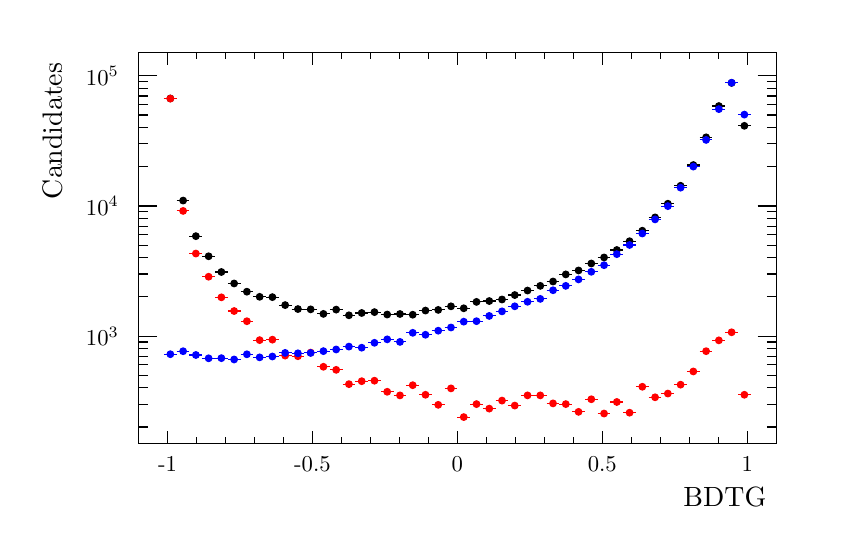
\begin{tikzpicture}
\pgfdeclareplotmark{cross} {
\pgfpathmoveto{\pgfpoint{-0.3\pgfplotmarksize}{\pgfplotmarksize}}
\pgfpathlineto{\pgfpoint{+0.3\pgfplotmarksize}{\pgfplotmarksize}}
\pgfpathlineto{\pgfpoint{+0.3\pgfplotmarksize}{0.3\pgfplotmarksize}}
\pgfpathlineto{\pgfpoint{+1\pgfplotmarksize}{0.3\pgfplotmarksize}}
\pgfpathlineto{\pgfpoint{+1\pgfplotmarksize}{-0.3\pgfplotmarksize}}
\pgfpathlineto{\pgfpoint{+0.3\pgfplotmarksize}{-0.3\pgfplotmarksize}}
\pgfpathlineto{\pgfpoint{+0.3\pgfplotmarksize}{-1.\pgfplotmarksize}}
\pgfpathlineto{\pgfpoint{-0.3\pgfplotmarksize}{-1.\pgfplotmarksize}}
\pgfpathlineto{\pgfpoint{-0.3\pgfplotmarksize}{-0.3\pgfplotmarksize}}
\pgfpathlineto{\pgfpoint{-1.\pgfplotmarksize}{-0.3\pgfplotmarksize}}
\pgfpathlineto{\pgfpoint{-1.\pgfplotmarksize}{0.3\pgfplotmarksize}}
\pgfpathlineto{\pgfpoint{-0.3\pgfplotmarksize}{0.3\pgfplotmarksize}}
\pgfpathclose
\pgfusepathqstroke
}
\pgfdeclareplotmark{cross*} {
\pgfpathmoveto{\pgfpoint{-0.3\pgfplotmarksize}{\pgfplotmarksize}}
\pgfpathlineto{\pgfpoint{+0.3\pgfplotmarksize}{\pgfplotmarksize}}
\pgfpathlineto{\pgfpoint{+0.3\pgfplotmarksize}{0.3\pgfplotmarksize}}
\pgfpathlineto{\pgfpoint{+1\pgfplotmarksize}{0.3\pgfplotmarksize}}
\pgfpathlineto{\pgfpoint{+1\pgfplotmarksize}{-0.3\pgfplotmarksize}}
\pgfpathlineto{\pgfpoint{+0.3\pgfplotmarksize}{-0.3\pgfplotmarksize}}
\pgfpathlineto{\pgfpoint{+0.3\pgfplotmarksize}{-1.\pgfplotmarksize}}
\pgfpathlineto{\pgfpoint{-0.3\pgfplotmarksize}{-1.\pgfplotmarksize}}
\pgfpathlineto{\pgfpoint{-0.3\pgfplotmarksize}{-0.3\pgfplotmarksize}}
\pgfpathlineto{\pgfpoint{-1.\pgfplotmarksize}{-0.3\pgfplotmarksize}}
\pgfpathlineto{\pgfpoint{-1.\pgfplotmarksize}{0.3\pgfplotmarksize}}
\pgfpathlineto{\pgfpoint{-0.3\pgfplotmarksize}{0.3\pgfplotmarksize}}
\pgfpathclose
\pgfusepathqfillstroke
}
\pgfdeclareplotmark{newstar} {
\pgfpathmoveto{\pgfqpoint{0pt}{\pgfplotmarksize}}
\pgfpathlineto{\pgfqpointpolar{44}{0.5\pgfplotmarksize}}
\pgfpathlineto{\pgfqpointpolar{18}{\pgfplotmarksize}}
\pgfpathlineto{\pgfqpointpolar{-20}{0.5\pgfplotmarksize}}
\pgfpathlineto{\pgfqpointpolar{-54}{\pgfplotmarksize}}
\pgfpathlineto{\pgfqpointpolar{-90}{0.5\pgfplotmarksize}}
\pgfpathlineto{\pgfqpointpolar{234}{\pgfplotmarksize}}
\pgfpathlineto{\pgfqpointpolar{198}{0.5\pgfplotmarksize}}
\pgfpathlineto{\pgfqpointpolar{162}{\pgfplotmarksize}}
\pgfpathlineto{\pgfqpointpolar{134}{0.5\pgfplotmarksize}}
\pgfpathclose
\pgfusepathqstroke
}
\pgfdeclareplotmark{newstar*} {
\pgfpathmoveto{\pgfqpoint{0pt}{\pgfplotmarksize}}
\pgfpathlineto{\pgfqpointpolar{44}{0.5\pgfplotmarksize}}
\pgfpathlineto{\pgfqpointpolar{18}{\pgfplotmarksize}}
\pgfpathlineto{\pgfqpointpolar{-20}{0.5\pgfplotmarksize}}
\pgfpathlineto{\pgfqpointpolar{-54}{\pgfplotmarksize}}
\pgfpathlineto{\pgfqpointpolar{-90}{0.5\pgfplotmarksize}}
\pgfpathlineto{\pgfqpointpolar{234}{\pgfplotmarksize}}
\pgfpathlineto{\pgfqpointpolar{198}{0.5\pgfplotmarksize}}
\pgfpathlineto{\pgfqpointpolar{162}{\pgfplotmarksize}}
\pgfpathlineto{\pgfqpointpolar{134}{0.5\pgfplotmarksize}}
\pgfpathclose
\pgfusepathqfillstroke
}
\definecolor{c}{rgb}{1,1,1};
\draw [color=c, fill=c] (0,0) rectangle (10,6.27517);
\draw [color=c, fill=c] (1.4,1.00403) rectangle (9.5,5.96141);
\definecolor{c}{rgb}{0,0,0};
\draw [c] (1.4,1.00403) -- (1.4,5.96141) -- (9.5,5.96141) -- (9.5,1.00403) -- (1.4,1.00403);
\draw [c,line width=0.4] (1.724,5.38328) -- (1.77144,5.38328);
\draw [c,line width=0.4] (1.83856,5.38328) -- (1.886,5.38328);
\foreach \P in {(1.805,5.38328)}{\draw[mark options={color=c,fill=c},mark size=1.201201pt,mark=*] plot coordinates {\P};}
\draw [c,line width=0.4] (1.886,4.08636) -- (1.93344,4.08636);
\draw [c,line width=0.4] (2.00056,4.08636) -- (2.048,4.08636);
\foreach \P in {(1.967,4.08636)}{\draw[mark options={color=c,fill=c},mark size=1.201201pt,mark=*] plot coordinates {\P};}
\draw [c,line width=0.4] (2.048,3.63442) -- (2.09544,3.63442);
\draw [c,line width=0.4] (2.16256,3.63442) -- (2.21,3.63442);
\foreach \P in {(2.129,3.63442)}{\draw[mark options={color=c,fill=c},mark size=1.201201pt,mark=*] plot coordinates {\P};}
\draw [c,line width=0.4] (2.21,3.37898) -- (2.25744,3.37898);
\draw [c,line width=0.4] (2.32456,3.37898) -- (2.372,3.37898);
\foreach \P in {(2.291,3.37898)}{\draw[mark options={color=c,fill=c},mark size=1.201201pt,mark=*] plot coordinates {\P};}
\draw [c,line width=0.4] (2.372,3.17931) -- (2.41944,3.17931);
\draw [c,line width=0.4] (2.48656,3.17931) -- (2.534,3.17931);
\foreach \P in {(2.453,3.17931)}{\draw[mark options={color=c,fill=c},mark size=1.201201pt,mark=*] plot coordinates {\P};}
\draw [c,line width=0.4] (2.534,3.03363) -- (2.58144,3.03363);
\draw [c,line width=0.4] (2.64856,3.03363) -- (2.696,3.03363);
\foreach \P in {(2.615,3.03363)}{\draw[mark options={color=c,fill=c},mark size=1.201201pt,mark=*] plot coordinates {\P};}
\draw [c,line width=0.4] (2.696,2.92906) -- (2.74344,2.92906);
\draw [c,line width=0.4] (2.81056,2.92906) -- (2.858,2.92906);
\foreach \P in {(2.777,2.92906)}{\draw[mark options={color=c,fill=c},mark size=1.201201pt,mark=*] plot coordinates {\P};}
\draw [c,line width=0.4] (2.858,2.86402) -- (2.90544,2.86402);
\draw [c,line width=0.4] (2.97256,2.86402) -- (3.02,2.86402);
\foreach \P in {(2.939,2.86402)}{\draw[mark options={color=c,fill=c},mark size=1.201201pt,mark=*] plot coordinates {\P};}
\draw [c,line width=0.4] (3.02,2.86007) -- (3.06744,2.86007);
\draw [c,line width=0.4] (3.13456,2.86007) -- (3.182,2.86007);
\foreach \P in {(3.101,2.86007)}{\draw[mark options={color=c,fill=c},mark size=1.201201pt,mark=*] plot coordinates {\P};}
\draw [c,line width=0.4] (3.182,2.75887) -- (3.22944,2.75887);
\draw [c,line width=0.4] (3.29656,2.75887) -- (3.344,2.75887);
\foreach \P in {(3.263,2.75887)}{\draw[mark options={color=c,fill=c},mark size=1.201201pt,mark=*] plot coordinates {\P};}
\draw [c,line width=0.4] (3.344,2.70861) -- (3.39144,2.70861);
\draw [c,line width=0.4] (3.45856,2.70861) -- (3.506,2.70861);
\foreach \P in {(3.425,2.70861)}{\draw[mark options={color=c,fill=c},mark size=1.201201pt,mark=*] plot coordinates {\P};}
\draw [c,line width=0.4] (3.506,2.7046) -- (3.55344,2.7046);
\draw [c,line width=0.4] (3.62056,2.7046) -- (3.668,2.7046);
\foreach \P in {(3.587,2.7046)}{\draw[mark options={color=c,fill=c},mark size=1.201201pt,mark=*] plot coordinates {\P};}
\draw [c,line width=0.4] (3.668,2.64734) -- (3.71544,2.64734);
\draw [c,line width=0.4] (3.78256,2.64734) -- (3.83,2.64734);
\foreach \P in {(3.749,2.64734)}{\draw[mark options={color=c,fill=c},mark size=1.201201pt,mark=*] plot coordinates {\P};}
\draw [c,line width=0.4] (3.83,2.70146) -- (3.87744,2.70146);
\draw [c,line width=0.4] (3.94456,2.70146) -- (3.992,2.70146);
\foreach \P in {(3.911,2.70146)}{\draw[mark options={color=c,fill=c},mark size=1.201201pt,mark=*] plot coordinates {\P};}
\draw [c,line width=0.4] (3.992,2.62918) -- (4.03944,2.62918);
\draw [c,line width=0.4] (4.10656,2.62918) -- (4.154,2.62918);
\foreach \P in {(4.073,2.62918)}{\draw[mark options={color=c,fill=c},mark size=1.201201pt,mark=*] plot coordinates {\P};}
\draw [c,line width=0.4] (4.154,2.65888) -- (4.20144,2.65888);
\draw [c,line width=0.4] (4.26856,2.65888) -- (4.316,2.65888);
\foreach \P in {(4.235,2.65888)}{\draw[mark options={color=c,fill=c},mark size=1.201201pt,mark=*] plot coordinates {\P};}
\draw [c,line width=0.4] (4.316,2.66976) -- (4.36344,2.66976);
\draw [c,line width=0.4] (4.43056,2.66976) -- (4.478,2.66976);
\foreach \P in {(4.397,2.66976)}{\draw[mark options={color=c,fill=c},mark size=1.201201pt,mark=*] plot coordinates {\P};}
\draw [c,line width=0.4] (4.478,2.63905) -- (4.52544,2.63905);
\draw [c,line width=0.4] (4.59256,2.63905) -- (4.64,2.63905);
\foreach \P in {(4.559,2.63905)}{\draw[mark options={color=c,fill=c},mark size=1.201201pt,mark=*] plot coordinates {\P};}
\draw [c,line width=0.4] (4.64,2.64588) -- (4.68744,2.64588);
\draw [c,line width=0.4] (4.75456,2.64588) -- (4.802,2.64588);
\foreach \P in {(4.721,2.64588)}{\draw[mark options={color=c,fill=c},mark size=1.201201pt,mark=*] plot coordinates {\P};}
\draw [c,line width=0.4] (4.802,2.6366) -- (4.84944,2.6366);
\draw [c,line width=0.4] (4.91656,2.6366) -- (4.964,2.6366);
\foreach \P in {(4.883,2.6366)}{\draw[mark options={color=c,fill=c},mark size=1.201201pt,mark=*] plot coordinates {\P};}
\draw [c,line width=0.4] (4.964,2.68968) -- (5.01144,2.68968);
\draw [c,line width=0.4] (5.07856,2.68968) -- (5.126,2.68968);
\foreach \P in {(5.045,2.68968)}{\draw[mark options={color=c,fill=c},mark size=1.201201pt,mark=*] plot coordinates {\P};}
\draw [c,line width=0.4] (5.126,2.69785) -- (5.17344,2.69785);
\draw [c,line width=0.4] (5.24056,2.69785) -- (5.288,2.69785);
\foreach \P in {(5.207,2.69785)}{\draw[mark options={color=c,fill=c},mark size=1.201201pt,mark=*] plot coordinates {\P};}
\draw [c,line width=0.4] (5.288,2.74335) -- (5.33544,2.74335);
\draw [c,line width=0.4] (5.40256,2.74335) -- (5.45,2.74335);
\foreach \P in {(5.369,2.74335)}{\draw[mark options={color=c,fill=c},mark size=1.201201pt,mark=*] plot coordinates {\P};}
\draw [c,line width=0.4] (5.45,2.71833) -- (5.49744,2.71833);
\draw [c,line width=0.4] (5.56456,2.71833) -- (5.612,2.71833);
\foreach \P in {(5.531,2.71833)}{\draw[mark options={color=c,fill=c},mark size=1.201201pt,mark=*] plot coordinates {\P};}
\draw [c,line width=0.4] (5.612,2.79959) -- (5.65944,2.79959);
\draw [c,line width=0.4] (5.72656,2.79959) -- (5.774,2.79959);
\foreach \P in {(5.693,2.79959)}{\draw[mark options={color=c,fill=c},mark size=1.201201pt,mark=*] plot coordinates {\P};}
\draw [c,line width=0.4] (5.774,2.81048) -- (5.82144,2.81048);
\draw [c,line width=0.4] (5.88856,2.81048) -- (5.936,2.81048);
\foreach \P in {(5.855,2.81048)}{\draw[mark options={color=c,fill=c},mark size=1.201201pt,mark=*] plot coordinates {\P};}
\draw [c,line width=0.4] (5.936,2.83028) -- (5.98344,2.83028);
\draw [c,line width=0.4] (6.05056,2.83028) -- (6.098,2.83028);
\foreach \P in {(6.017,2.83028)}{\draw[mark options={color=c,fill=c},mark size=1.201201pt,mark=*] plot coordinates {\P};}
\draw [c,line width=0.4] (6.098,2.88659) -- (6.14544,2.88659);
\draw [c,line width=0.4] (6.21256,2.88659) -- (6.26,2.88659);
\foreach \P in {(6.179,2.88659)}{\draw[mark options={color=c,fill=c},mark size=1.201201pt,mark=*] plot coordinates {\P};}
\draw [c,line width=0.4] (6.26,2.94395) -- (6.30744,2.94395);
\draw [c,line width=0.4] (6.37456,2.94395) -- (6.422,2.94395);
\foreach \P in {(6.341,2.94395)}{\draw[mark options={color=c,fill=c},mark size=1.201201pt,mark=*] plot coordinates {\P};}
\draw [c,line width=0.4] (6.422,3.00329) -- (6.46944,3.00329);
\draw [c,line width=0.4] (6.53656,3.00329) -- (6.584,3.00329);
\foreach \P in {(6.503,3.00329)}{\draw[mark options={color=c,fill=c},mark size=1.201201pt,mark=*] plot coordinates {\P};}
\draw [c,line width=0.4] (6.584,3.05837) -- (6.63144,3.05837);
\draw [c,line width=0.4] (6.69856,3.05837) -- (6.746,3.05837);
\foreach \P in {(6.665,3.05837)}{\draw[mark options={color=c,fill=c},mark size=1.201201pt,mark=*] plot coordinates {\P};}
\draw [c,line width=0.4] (6.746,3.14889) -- (6.79344,3.14889);
\draw [c,line width=0.4] (6.86056,3.14889) -- (6.908,3.14889);
\foreach \P in {(6.827,3.14889)}{\draw[mark options={color=c,fill=c},mark size=1.201201pt,mark=*] plot coordinates {\P};}
\draw [c,line width=0.4] (6.908,3.1989) -- (6.95544,3.1989);
\draw [c,line width=0.4] (7.02256,3.1989) -- (7.07,3.1989);
\foreach \P in {(6.989,3.1989)}{\draw[mark options={color=c,fill=c},mark size=1.201201pt,mark=*] plot coordinates {\P};}
\draw [c,line width=0.4] (7.07,3.28736) -- (7.11744,3.28736);
\draw [c,line width=0.4] (7.18456,3.28736) -- (7.232,3.28736);
\foreach \P in {(7.151,3.28736)}{\draw[mark options={color=c,fill=c},mark size=1.201201pt,mark=*] plot coordinates {\P};}
\draw [c,line width=0.4] (7.232,3.36396) -- (7.27944,3.36396);
\draw [c,line width=0.4] (7.34656,3.36396) -- (7.394,3.36396);
\foreach \P in {(7.313,3.36396)}{\draw[mark options={color=c,fill=c},mark size=1.201201pt,mark=*] plot coordinates {\P};}
\draw [c,line width=0.4] (7.394,3.45865) -- (7.44144,3.45865);
\draw [c,line width=0.4] (7.50856,3.45865) -- (7.556,3.45865);
\foreach \P in {(7.475,3.45865)}{\draw[mark options={color=c,fill=c},mark size=1.201201pt,mark=*] plot coordinates {\P};}
\draw [c,line width=0.4] (7.556,3.57029) -- (7.60344,3.57029);
\draw [c,line width=0.4] (7.67056,3.57029) -- (7.718,3.57029);
\foreach \P in {(7.637,3.57029)}{\draw[mark options={color=c,fill=c},mark size=1.201201pt,mark=*] plot coordinates {\P};}
\draw [c,line width=0.4] (7.718,3.70349) -- (7.76544,3.70349);
\draw [c,line width=0.4] (7.83256,3.70349) -- (7.88,3.70349);
\foreach \P in {(7.799,3.70349)}{\draw[mark options={color=c,fill=c},mark size=1.201201pt,mark=*] plot coordinates {\P};}
\draw [c,line width=0.4] (7.88,3.87256) -- (7.92744,3.87256);
\draw [c,line width=0.4] (7.99456,3.87256) -- (8.042,3.87256);
\foreach \P in {(7.961,3.87256)}{\draw[mark options={color=c,fill=c},mark size=1.201201pt,mark=*] plot coordinates {\P};}
\draw [c,line width=0.4] (8.042,4.04625) -- (8.08944,4.04625);
\draw [c,line width=0.4] (8.15656,4.04625) -- (8.204,4.04625);
\foreach \P in {(8.123,4.04625)}{\draw[mark options={color=c,fill=c},mark size=1.201201pt,mark=*] plot coordinates {\P};}
\draw [c,line width=0.4] (8.204,4.27415) -- (8.25144,4.27415);
\draw [c,line width=0.4] (8.31856,4.27415) -- (8.366,4.27415);
\foreach \P in {(8.285,4.27415)}{\draw[mark options={color=c,fill=c},mark size=1.201201pt,mark=*] plot coordinates {\P};}
\draw [c,line width=0.4] (8.366,4.53756) -- (8.41344,4.53756);
\draw [c,line width=0.4] (8.48056,4.53756) -- (8.528,4.53756);
\foreach \P in {(8.447,4.53756)}{\draw[mark options={color=c,fill=c},mark size=1.201201pt,mark=*] plot coordinates {\P};}
\draw [c,line width=0.4] (8.528,4.88958) -- (8.57544,4.88958);
\draw [c,line width=0.4] (8.64256,4.88958) -- (8.69,4.88958);
\foreach \P in {(8.609,4.88958)}{\draw[mark options={color=c,fill=c},mark size=1.201201pt,mark=*] plot coordinates {\P};}
\draw [c,line width=0.4] (8.69,5.28678) -- (8.73744,5.28678);
\draw [c,line width=0.4] (8.80456,5.28678) -- (8.852,5.28678);
\foreach \P in {(8.771,5.28678)}{\draw[mark options={color=c,fill=c},mark size=1.201201pt,mark=*] plot coordinates {\P};}
\draw [c,line width=0.4] (8.852,5.58057) -- (8.89944,5.58057);
\draw [c,line width=0.4] (8.96656,5.58057) -- (9.014,5.58057);
\foreach \P in {(8.933,5.58057)}{\draw[mark options={color=c,fill=c},mark size=1.201201pt,mark=*] plot coordinates {\P};}
\draw [c,line width=0.4] (9.014,5.03564) -- (9.06144,5.03564);
\draw [c,line width=0.4] (9.12856,5.03564) -- (9.176,5.03564);
\foreach \P in {(9.095,5.03564)}{\draw[mark options={color=c,fill=c},mark size=1.201201pt,mark=*] plot coordinates {\P};}
\draw [c,line width=0.4] (1.4,1.00403) -- (9.5,1.00403);
\draw [anchor= east] (9.5,0.317272) node[scale=1.00614, rotate=0]{BDTG};
\draw [c,line width=0.4] (1.76818,1.15651) -- (1.76818,1.00403);
\draw [c,line width=0.4] (2.13636,1.08027) -- (2.13636,1.00403);
\draw [c,line width=0.4] (2.50455,1.08027) -- (2.50455,1.00403);
\draw [c,line width=0.4] (2.87273,1.08027) -- (2.87273,1.00403);
\draw [c,line width=0.4] (3.24091,1.08027) -- (3.24091,1.00403);
\draw [c,line width=0.4] (3.60909,1.15651) -- (3.60909,1.00403);
\draw [c,line width=0.4] (3.97727,1.08027) -- (3.97727,1.00403);
\draw [c,line width=0.4] (4.34545,1.08027) -- (4.34545,1.00403);
\draw [c,line width=0.4] (4.71364,1.08027) -- (4.71364,1.00403);
\draw [c,line width=0.4] (5.08182,1.08027) -- (5.08182,1.00403);
\draw [c,line width=0.4] (5.45,1.15651) -- (5.45,1.00403);
\draw [c,line width=0.4] (5.81818,1.08027) -- (5.81818,1.00403);
\draw [c,line width=0.4] (6.18636,1.08027) -- (6.18636,1.00403);
\draw [c,line width=0.4] (6.55455,1.08027) -- (6.55455,1.00403);
\draw [c,line width=0.4] (6.92273,1.08027) -- (6.92273,1.00403);
\draw [c,line width=0.4] (7.29091,1.15651) -- (7.29091,1.00403);
\draw [c,line width=0.4] (7.65909,1.08027) -- (7.65909,1.00403);
\draw [c,line width=0.4] (8.02727,1.08027) -- (8.02727,1.00403);
\draw [c,line width=0.4] (8.39545,1.08027) -- (8.39545,1.00403);
\draw [c,line width=0.4] (8.76364,1.08027) -- (8.76364,1.00403);
\draw [c,line width=0.4] (9.13182,1.15651) -- (9.13182,1.00403);
\draw [c,line width=0.4] (1.76818,1.15651) -- (1.76818,1.00403);
\draw [c,line width=0.4] (1.4,1.08027) -- (1.4,1.00403);
\draw [c,line width=0.4] (9.13182,1.15651) -- (9.13182,1.00403);
\draw [c,line width=0.4] (9.5,1.08027) -- (9.5,1.00403);
\draw [anchor=base] (1.76818,0.640067) node[scale=0.819821, rotate=0]{-1};
\draw [anchor=base] (3.60909,0.640067) node[scale=0.819821, rotate=0]{-0.5};
\draw [anchor=base] (5.45,0.640067) node[scale=0.819821, rotate=0]{0};
\draw [anchor=base] (7.29091,0.640067) node[scale=0.819821, rotate=0]{0.5};
\draw [anchor=base] (9.13182,0.640067) node[scale=0.819821, rotate=0]{1};
\draw [c,line width=0.4] (1.4,5.96141) -- (9.5,5.96141);
\draw [c,line width=0.4] (1.76818,5.80892) -- (1.76818,5.96141);
\draw [c,line width=0.4] (2.13636,5.88517) -- (2.13636,5.96141);
\draw [c,line width=0.4] (2.50455,5.88517) -- (2.50455,5.96141);
\draw [c,line width=0.4] (2.87273,5.88517) -- (2.87273,5.96141);
\draw [c,line width=0.4] (3.24091,5.88517) -- (3.24091,5.96141);
\draw [c,line width=0.4] (3.60909,5.80892) -- (3.60909,5.96141);
\draw [c,line width=0.4] (3.97727,5.88517) -- (3.97727,5.96141);
\draw [c,line width=0.4] (4.34545,5.88517) -- (4.34545,5.96141);
\draw [c,line width=0.4] (4.71364,5.88517) -- (4.71364,5.96141);
\draw [c,line width=0.4] (5.08182,5.88517) -- (5.08182,5.96141);
\draw [c,line width=0.4] (5.45,5.80892) -- (5.45,5.96141);
\draw [c,line width=0.4] (5.81818,5.88517) -- (5.81818,5.96141);
\draw [c,line width=0.4] (6.18636,5.88517) -- (6.18636,5.96141);
\draw [c,line width=0.4] (6.55455,5.88517) -- (6.55455,5.96141);
\draw [c,line width=0.4] (6.92273,5.88517) -- (6.92273,5.96141);
\draw [c,line width=0.4] (7.29091,5.80892) -- (7.29091,5.96141);
\draw [c,line width=0.4] (7.65909,5.88517) -- (7.65909,5.96141);
\draw [c,line width=0.4] (8.02727,5.88517) -- (8.02727,5.96141);
\draw [c,line width=0.4] (8.39545,5.88517) -- (8.39545,5.96141);
\draw [c,line width=0.4] (8.76364,5.88517) -- (8.76364,5.96141);
\draw [c,line width=0.4] (9.13182,5.80892) -- (9.13182,5.96141);
\draw [c,line width=0.4] (1.76818,5.80892) -- (1.76818,5.96141);
\draw [c,line width=0.4] (1.4,5.88517) -- (1.4,5.96141);
\draw [c,line width=0.4] (9.13182,5.80892) -- (9.13182,5.96141);
\draw [c,line width=0.4] (9.5,5.88517) -- (9.5,5.96141);
\draw [c,line width=0.4] (1.4,1.00403) -- (1.4,5.96141);
\draw [anchor= east] (0.3056,5.96141) node[scale=1.00614, rotate=90]{Candidates};
\draw [c,line width=0.4] (1.5185,1.21048) -- (1.4,1.21048);
\draw [c,line width=0.4] (1.5185,1.50147) -- (1.4,1.50147);
\draw [c,line width=0.4] (1.5185,1.70792) -- (1.4,1.70792);
\draw [c,line width=0.4] (1.5185,1.86806) -- (1.4,1.86806);
\draw [c,line width=0.4] (1.5185,1.99891) -- (1.4,1.99891);
\draw [c,line width=0.4] (1.5185,2.10953) -- (1.4,2.10953);
\draw [c,line width=0.4] (1.5185,2.20536) -- (1.4,2.20536);
\draw [c,line width=0.4] (1.5185,2.28989) -- (1.4,2.28989);
\draw [c,line width=0.4] (1.637,2.3655) -- (1.4,2.3655);
\draw [anchor= east] (1.252,2.3655) node[scale=0.819821, rotate=0]{$10^{3}$};
\draw [c,line width=0.4] (1.5185,2.86294) -- (1.4,2.86294);
\draw [c,line width=0.4] (1.5185,3.15393) -- (1.4,3.15393);
\draw [c,line width=0.4] (1.5185,3.36038) -- (1.4,3.36038);
\draw [c,line width=0.4] (1.5185,3.52052) -- (1.4,3.52052);
\draw [c,line width=0.4] (1.5185,3.65137) -- (1.4,3.65137);
\draw [c,line width=0.4] (1.5185,3.76199) -- (1.4,3.76199);
\draw [c,line width=0.4] (1.5185,3.85782) -- (1.4,3.85782);
\draw [c,line width=0.4] (1.5185,3.94235) -- (1.4,3.94235);
\draw [c,line width=0.4] (1.637,4.01796) -- (1.4,4.01796);
\draw [anchor= east] (1.252,4.01796) node[scale=0.819821, rotate=0]{$10^{4}$};
\draw [c,line width=0.4] (1.5185,4.5154) -- (1.4,4.5154);
\draw [c,line width=0.4] (1.5185,4.80639) -- (1.4,4.80639);
\draw [c,line width=0.4] (1.5185,5.01285) -- (1.4,5.01285);
\draw [c,line width=0.4] (1.5185,5.17299) -- (1.4,5.17299);
\draw [c,line width=0.4] (1.5185,5.30383) -- (1.4,5.30383);
\draw [c,line width=0.4] (1.5185,5.41446) -- (1.4,5.41446);
\draw [c,line width=0.4] (1.5185,5.51029) -- (1.4,5.51029);
\draw [c,line width=0.4] (1.5185,5.59481) -- (1.4,5.59481);
\draw [c,line width=0.4] (1.637,5.67043) -- (1.4,5.67043);
\draw [anchor= east] (1.252,5.67043) node[scale=0.819821, rotate=0]{$10^{5}$};
\draw [c,line width=0.4] (9.5,1.00403) -- (9.5,5.96141);
\draw [c,line width=0.4] (9.3815,1.21048) -- (9.5,1.21048);
\draw [c,line width=0.4] (9.3815,1.50147) -- (9.5,1.50147);
\draw [c,line width=0.4] (9.3815,1.70792) -- (9.5,1.70792);
\draw [c,line width=0.4] (9.3815,1.86806) -- (9.5,1.86806);
\draw [c,line width=0.4] (9.3815,1.99891) -- (9.5,1.99891);
\draw [c,line width=0.4] (9.3815,2.10953) -- (9.5,2.10953);
\draw [c,line width=0.4] (9.3815,2.20536) -- (9.5,2.20536);
\draw [c,line width=0.4] (9.3815,2.28989) -- (9.5,2.28989);
\draw [c,line width=0.4] (9.263,2.3655) -- (9.5,2.3655);
\draw [c,line width=0.4] (9.3815,2.86294) -- (9.5,2.86294);
\draw [c,line width=0.4] (9.3815,3.15393) -- (9.5,3.15393);
\draw [c,line width=0.4] (9.3815,3.36038) -- (9.5,3.36038);
\draw [c,line width=0.4] (9.3815,3.52052) -- (9.5,3.52052);
\draw [c,line width=0.4] (9.3815,3.65137) -- (9.5,3.65137);
\draw [c,line width=0.4] (9.3815,3.76199) -- (9.5,3.76199);
\draw [c,line width=0.4] (9.3815,3.85782) -- (9.5,3.85782);
\draw [c,line width=0.4] (9.3815,3.94235) -- (9.5,3.94235);
\draw [c,line width=0.4] (9.263,4.01796) -- (9.5,4.01796);
\draw [c,line width=0.4] (9.3815,4.5154) -- (9.5,4.5154);
\draw [c,line width=0.4] (9.3815,4.80639) -- (9.5,4.80639);
\draw [c,line width=0.4] (9.3815,5.01285) -- (9.5,5.01285);
\draw [c,line width=0.4] (9.3815,5.17299) -- (9.5,5.17299);
\draw [c,line width=0.4] (9.3815,5.30383) -- (9.5,5.30383);
\draw [c,line width=0.4] (9.3815,5.41446) -- (9.5,5.41446);
\draw [c,line width=0.4] (9.3815,5.51029) -- (9.5,5.51029);
\draw [c,line width=0.4] (9.3815,5.59481) -- (9.5,5.59481);
\draw [c,line width=0.4] (9.263,5.67043) -- (9.5,5.67043);
\definecolor{c}{rgb}{1,0,0};
\draw [c,line width=0.4] (1.724,5.38163) -- (1.77144,5.38163);
\draw [c,line width=0.4] (1.83856,5.38163) -- (1.886,5.38163);
\foreach \P in {(1.805,5.38163)}{\draw[mark options={color=c,fill=c},mark size=1.201201pt,mark=*] plot coordinates {\P};}
\draw [c,line width=0.4] (1.886,3.95491) -- (1.93344,3.95491);
\draw [c,line width=0.4] (2.00056,3.95491) -- (2.048,3.95491);
\foreach \P in {(1.967,3.95491)}{\draw[mark options={color=c,fill=c},mark size=1.201201pt,mark=*] plot coordinates {\P};}
\draw [c,line width=0.4] (2.048,3.41366) -- (2.09544,3.41366);
\draw [c,line width=0.4] (2.16256,3.41366) -- (2.21,3.41366);
\foreach \P in {(2.129,3.41366)}{\draw[mark options={color=c,fill=c},mark size=1.201201pt,mark=*] plot coordinates {\P};}
\draw [c,line width=0.4] (2.21,3.11914) -- (2.25744,3.11914);
\draw [c,line width=0.4] (2.32456,3.11914) -- (2.372,3.11914);
\foreach \P in {(2.291,3.11914)}{\draw[mark options={color=c,fill=c},mark size=1.201201pt,mark=*] plot coordinates {\P};}
\draw [c,line width=0.4] (2.372,2.85749) -- (2.41944,2.85749);
\draw [c,line width=0.4] (2.48656,2.85749) -- (2.534,2.85749);
\foreach \P in {(2.453,2.85749)}{\draw[mark options={color=c,fill=c},mark size=1.201201pt,mark=*] plot coordinates {\P};}
\draw [c,line width=0.4] (2.534,2.68366) -- (2.58144,2.68366);
\draw [c,line width=0.4] (2.64856,2.68366) -- (2.696,2.68366);
\foreach \P in {(2.615,2.68366)}{\draw[mark options={color=c,fill=c},mark size=1.201201pt,mark=*] plot coordinates {\P};}
\draw [c,line width=0.4] (2.696,2.55388) -- (2.74344,2.55388);
\draw [c,line width=0.4] (2.81056,2.55388) -- (2.858,2.55388);
\foreach \P in {(2.777,2.55388)}{\draw[mark options={color=c,fill=c},mark size=1.201201pt,mark=*] plot coordinates {\P};}
\draw [c,line width=0.4] (2.858,2.31411) -- (2.90544,2.31411);
\draw [c,line width=0.4] (2.97256,2.31411) -- (3.02,2.31411);
\foreach \P in {(2.939,2.31411)}{\draw[mark options={color=c,fill=c},mark size=1.201201pt,mark=*] plot coordinates {\P};}
\draw [c,line width=0.4] (3.02,2.32001) -- (3.06744,2.32001);
\draw [c,line width=0.4] (3.13456,2.32001) -- (3.182,2.32001);
\foreach \P in {(3.101,2.32001)}{\draw[mark options={color=c,fill=c},mark size=1.201201pt,mark=*] plot coordinates {\P};}
\draw [c,line width=0.4] (3.182,2.11747) -- (3.22944,2.11747);
\draw [c,line width=0.4] (3.29656,2.11747) -- (3.344,2.11747);
\foreach \P in {(3.263,2.11747)}{\draw[mark options={color=c,fill=c},mark size=1.201201pt,mark=*] plot coordinates {\P};}
\draw [c,line width=0.4] (3.344,2.10962) -- (3.39144,2.10962);
\draw [c,line width=0.4] (3.45856,2.10962) -- (3.506,2.10962);
\foreach \P in {(3.425,2.10962)}{\draw[mark options={color=c,fill=c},mark size=1.201201pt,mark=*] plot coordinates {\P};}
\draw [c,line width=0.4] (3.506,2.15545) -- (3.55344,2.15545);
\draw [c,line width=0.4] (3.62056,2.15545) -- (3.668,2.15545);
\foreach \P in {(3.587,2.15545)}{\draw[mark options={color=c,fill=c},mark size=1.201201pt,mark=*] plot coordinates {\P};}
\draw [c,line width=0.4] (3.668,1.97562) -- (3.71544,1.97562);
\draw [c,line width=0.4] (3.78256,1.97562) -- (3.83,1.97562);
\foreach \P in {(3.749,1.97562)}{\draw[mark options={color=c,fill=c},mark size=1.201201pt,mark=*] plot coordinates {\P};}
\draw [c,line width=0.4] (3.83,1.93655) -- (3.87744,1.93655);
\draw [c,line width=0.4] (3.94456,1.93655) -- (3.992,1.93655);
\foreach \P in {(3.911,1.93655)}{\draw[mark options={color=c,fill=c},mark size=1.201201pt,mark=*] plot coordinates {\P};}
\draw [c,line width=0.4] (4.073,1.71916) -- (4.073,1.7212);
\draw [c,line width=0.4] (4.073,1.78832) -- (4.073,1.78868);
\draw [c,line width=0.4] (3.992,1.75476) -- (4.03944,1.75476);
\draw [c,line width=0.4] (4.10656,1.75476) -- (4.154,1.75476);
\foreach \P in {(4.073,1.75476)}{\draw[mark options={color=c,fill=c},mark size=1.201201pt,mark=*] plot coordinates {\P};}
\draw [c,line width=0.4] (4.235,1.75789) -- (4.235,1.75898);
\draw [c,line width=0.4] (4.154,1.79254) -- (4.20144,1.79254);
\draw [c,line width=0.4] (4.26856,1.79254) -- (4.316,1.79254);
\foreach \P in {(4.235,1.79254)}{\draw[mark options={color=c,fill=c},mark size=1.201201pt,mark=*] plot coordinates {\P};}
\draw [c,line width=0.4] (4.397,1.76415) -- (4.397,1.76509);
\draw [c,line width=0.4] (4.316,1.79865) -- (4.36344,1.79865);
\draw [c,line width=0.4] (4.43056,1.79865) -- (4.478,1.79865);
\foreach \P in {(4.397,1.79865)}{\draw[mark options={color=c,fill=c},mark size=1.201201pt,mark=*] plot coordinates {\P};}
\draw [c,line width=0.4] (4.559,1.61986) -- (4.559,1.62445);
\draw [c,line width=0.4] (4.559,1.69156) -- (4.559,1.69423);
\draw [c,line width=0.4] (4.478,1.65801) -- (4.52544,1.65801);
\draw [c,line width=0.4] (4.59256,1.65801) -- (4.64,1.65801);
\foreach \P in {(4.559,1.65801)}{\draw[mark options={color=c,fill=c},mark size=1.201201pt,mark=*] plot coordinates {\P};}
\draw [c,line width=0.4] (4.721,1.57276) -- (4.721,1.57863);
\draw [c,line width=0.4] (4.721,1.64574) -- (4.721,1.64955);
\draw [c,line width=0.4] (4.64,1.61218) -- (4.68744,1.61218);
\draw [c,line width=0.4] (4.75456,1.61218) -- (4.802,1.61218);
\foreach \P in {(4.721,1.61218)}{\draw[mark options={color=c,fill=c},mark size=1.201201pt,mark=*] plot coordinates {\P};}
\draw [c,line width=0.4] (4.883,1.70578) -- (4.883,1.70816);
\draw [c,line width=0.4] (4.883,1.77527) -- (4.883,1.77593);
\draw [c,line width=0.4] (4.802,1.74171) -- (4.84944,1.74171);
\draw [c,line width=0.4] (4.91656,1.74171) -- (4.964,1.74171);
\foreach \P in {(4.883,1.74171)}{\draw[mark options={color=c,fill=c},mark size=1.201201pt,mark=*] plot coordinates {\P};}
\draw [c,line width=0.4] (5.045,1.58083) -- (5.045,1.58647);
\draw [c,line width=0.4] (5.045,1.65358) -- (5.045,1.6572);
\draw [c,line width=0.4] (4.964,1.62003) -- (5.01144,1.62003);
\draw [c,line width=0.4] (5.07856,1.62003) -- (5.126,1.62003);
\foreach \P in {(5.045,1.62003)}{\draw[mark options={color=c,fill=c},mark size=1.201201pt,mark=*] plot coordinates {\P};}
\draw [c,line width=0.4] (5.207,1.44934) -- (5.207,1.45874);
\draw [c,line width=0.4] (5.207,1.52585) -- (5.207,1.53283);
\draw [c,line width=0.4] (5.126,1.4923) -- (5.17344,1.4923);
\draw [c,line width=0.4] (5.24056,1.4923) -- (5.288,1.4923);
\foreach \P in {(5.207,1.4923)}{\draw[mark options={color=c,fill=c},mark size=1.201201pt,mark=*] plot coordinates {\P};}
\draw [c,line width=0.4] (5.369,1.66409) -- (5.369,1.66752);
\draw [c,line width=0.4] (5.369,1.73464) -- (5.369,1.73626);
\draw [c,line width=0.4] (5.288,1.70108) -- (5.33544,1.70108);
\draw [c,line width=0.4] (5.40256,1.70108) -- (5.45,1.70108);
\foreach \P in {(5.369,1.70108)}{\draw[mark options={color=c,fill=c},mark size=1.201201pt,mark=*] plot coordinates {\P};}
\draw [c,line width=0.4] (5.531,1.28876) -- (5.531,1.30325);
\draw [c,line width=0.4] (5.531,1.37036) -- (5.531,1.38183);
\draw [c,line width=0.4] (5.45,1.3368) -- (5.49744,1.3368);
\draw [c,line width=0.4] (5.56456,1.3368) -- (5.612,1.3368);
\foreach \P in {(5.531,1.3368)}{\draw[mark options={color=c,fill=c},mark size=1.201201pt,mark=*] plot coordinates {\P};}
\draw [c,line width=0.4] (5.693,1.45888) -- (5.693,1.468);
\draw [c,line width=0.4] (5.693,1.53511) -- (5.693,1.54184);
\draw [c,line width=0.4] (5.612,1.50156) -- (5.65944,1.50156);
\draw [c,line width=0.4] (5.72656,1.50156) -- (5.774,1.50156);
\foreach \P in {(5.693,1.50156)}{\draw[mark options={color=c,fill=c},mark size=1.201201pt,mark=*] plot coordinates {\P};}
\draw [c,line width=0.4] (5.855,1.39964) -- (5.855,1.41056);
\draw [c,line width=0.4] (5.855,1.47767) -- (5.855,1.48599);
\draw [c,line width=0.4] (5.774,1.44411) -- (5.82144,1.44411);
\draw [c,line width=0.4] (5.88856,1.44411) -- (5.936,1.44411);
\foreach \P in {(5.855,1.44411)}{\draw[mark options={color=c,fill=c},mark size=1.201201pt,mark=*] plot coordinates {\P};}
\draw [c,line width=0.4] (6.017,1.50481) -- (6.017,1.51259);
\draw [c,line width=0.4] (6.017,1.5797) -- (6.017,1.58523);
\draw [c,line width=0.4] (5.936,1.54615) -- (5.98344,1.54615);
\draw [c,line width=0.4] (6.05056,1.54615) -- (6.098,1.54615);
\foreach \P in {(6.017,1.54615)}{\draw[mark options={color=c,fill=c},mark size=1.201201pt,mark=*] plot coordinates {\P};}
\draw [c,line width=0.4] (6.179,1.43967) -- (6.179,1.44936);
\draw [c,line width=0.4] (6.179,1.51647) -- (6.179,1.52371);
\draw [c,line width=0.4] (6.098,1.48292) -- (6.14544,1.48292);
\draw [c,line width=0.4] (6.21256,1.48292) -- (6.26,1.48292);
\foreach \P in {(6.179,1.48292)}{\draw[mark options={color=c,fill=c},mark size=1.201201pt,mark=*] plot coordinates {\P};}
\draw [c,line width=0.4] (6.341,1.57276) -- (6.341,1.57863);
\draw [c,line width=0.4] (6.341,1.64574) -- (6.341,1.64955);
\draw [c,line width=0.4] (6.26,1.61218) -- (6.30744,1.61218);
\draw [c,line width=0.4] (6.37456,1.61218) -- (6.422,1.61218);
\foreach \P in {(6.341,1.61218)}{\draw[mark options={color=c,fill=c},mark size=1.201201pt,mark=*] plot coordinates {\P};}
\draw [c,line width=0.4] (6.503,1.57276) -- (6.503,1.57863);
\draw [c,line width=0.4] (6.503,1.64574) -- (6.503,1.64955);
\draw [c,line width=0.4] (6.422,1.61218) -- (6.46944,1.61218);
\draw [c,line width=0.4] (6.53656,1.61218) -- (6.584,1.61218);
\foreach \P in {(6.503,1.61218)}{\draw[mark options={color=c,fill=c},mark size=1.201201pt,mark=*] plot coordinates {\P};}
\draw [c,line width=0.4] (6.665,1.4683) -- (6.665,1.47714);
\draw [c,line width=0.4] (6.665,1.54426) -- (6.665,1.55073);
\draw [c,line width=0.4] (6.584,1.5107) -- (6.63144,1.5107);
\draw [c,line width=0.4] (6.69856,1.5107) -- (6.746,1.5107);
\foreach \P in {(6.665,1.5107)}{\draw[mark options={color=c,fill=c},mark size=1.201201pt,mark=*] plot coordinates {\P};}
\draw [c,line width=0.4] (6.827,1.45888) -- (6.827,1.468);
\draw [c,line width=0.4] (6.827,1.53511) -- (6.827,1.54184);
\draw [c,line width=0.4] (6.746,1.50156) -- (6.79344,1.50156);
\draw [c,line width=0.4] (6.86056,1.50156) -- (6.908,1.50156);
\foreach \P in {(6.827,1.50156)}{\draw[mark options={color=c,fill=c},mark size=1.201201pt,mark=*] plot coordinates {\P};}
\draw [c,line width=0.4] (6.989,1.35729) -- (6.989,1.36954);
\draw [c,line width=0.4] (6.989,1.43665) -- (6.989,1.44615);
\draw [c,line width=0.4] (6.908,1.40309) -- (6.95544,1.40309);
\draw [c,line width=0.4] (7.02256,1.40309) -- (7.07,1.40309);
\foreach \P in {(6.989,1.40309)}{\draw[mark options={color=c,fill=c},mark size=1.201201pt,mark=*] plot coordinates {\P};}
\draw [c,line width=0.4] (7.151,1.52241) -- (7.151,1.52968);
\draw [c,line width=0.4] (7.151,1.59679) -- (7.151,1.60186);
\draw [c,line width=0.4] (7.07,1.56323) -- (7.11744,1.56323);
\draw [c,line width=0.4] (7.18456,1.56323) -- (7.232,1.56323);
\foreach \P in {(7.151,1.56323)}{\draw[mark options={color=c,fill=c},mark size=1.201201pt,mark=*] plot coordinates {\P};}
\draw [c,line width=0.4] (7.313,1.33515) -- (7.313,1.34811);
\draw [c,line width=0.4] (7.313,1.41523) -- (7.313,1.42535);
\draw [c,line width=0.4] (7.232,1.38167) -- (7.27944,1.38167);
\draw [c,line width=0.4] (7.34656,1.38167) -- (7.394,1.38167);
\foreach \P in {(7.313,1.38167)}{\draw[mark options={color=c,fill=c},mark size=1.201201pt,mark=*] plot coordinates {\P};}
\draw [c,line width=0.4] (7.475,1.48679) -- (7.475,1.49508);
\draw [c,line width=0.4] (7.475,1.5622) -- (7.475,1.56819);
\draw [c,line width=0.4] (7.394,1.52864) -- (7.44144,1.52864);
\draw [c,line width=0.4] (7.50856,1.52864) -- (7.556,1.52864);
\foreach \P in {(7.475,1.52864)}{\draw[mark options={color=c,fill=c},mark size=1.201201pt,mark=*] plot coordinates {\P};}
\draw [c,line width=0.4] (7.637,1.34631) -- (7.637,1.35891);
\draw [c,line width=0.4] (7.637,1.42602) -- (7.637,1.43583);
\draw [c,line width=0.4] (7.556,1.39246) -- (7.60344,1.39246);
\draw [c,line width=0.4] (7.67056,1.39246) -- (7.718,1.39246);
\foreach \P in {(7.637,1.39246)}{\draw[mark options={color=c,fill=c},mark size=1.201201pt,mark=*] plot coordinates {\P};}
\draw [c,line width=0.4] (7.799,1.68523) -- (7.799,1.68813);
\draw [c,line width=0.4] (7.799,1.75524) -- (7.799,1.75637);
\draw [c,line width=0.4] (7.718,1.72168) -- (7.76544,1.72168);
\draw [c,line width=0.4] (7.83256,1.72168) -- (7.88,1.72168);
\foreach \P in {(7.799,1.72168)}{\draw[mark options={color=c,fill=c},mark size=1.201201pt,mark=*] plot coordinates {\P};}
\draw [c,line width=0.4] (7.961,1.54802) -- (7.961,1.55457);
\draw [c,line width=0.4] (7.961,1.62168) -- (7.961,1.62611);
\draw [c,line width=0.4] (7.88,1.58813) -- (7.92744,1.58813);
\draw [c,line width=0.4] (7.99456,1.58813) -- (8.042,1.58813);
\foreach \P in {(7.961,1.58813)}{\draw[mark options={color=c,fill=c},mark size=1.201201pt,mark=*] plot coordinates {\P};}
\draw [c,line width=0.4] (8.123,1.59669) -- (8.123,1.6019);
\draw [c,line width=0.4] (8.123,1.66902) -- (8.123,1.67224);
\draw [c,line width=0.4] (8.042,1.63546) -- (8.08944,1.63546);
\draw [c,line width=0.4] (8.15656,1.63546) -- (8.204,1.63546);
\foreach \P in {(8.123,1.63546)}{\draw[mark options={color=c,fill=c},mark size=1.201201pt,mark=*] plot coordinates {\P};}
\draw [c,line width=0.4] (8.285,1.7125) -- (8.285,1.71471);
\draw [c,line width=0.4] (8.285,1.78182) -- (8.285,1.78233);
\draw [c,line width=0.4] (8.204,1.74827) -- (8.25144,1.74827);
\draw [c,line width=0.4] (8.31856,1.74827) -- (8.366,1.74827);
\foreach \P in {(8.285,1.74827)}{\draw[mark options={color=c,fill=c},mark size=1.201201pt,mark=*] plot coordinates {\P};}
\draw [c,line width=0.4] (8.366,1.91619) -- (8.41344,1.91619);
\draw [c,line width=0.4] (8.48056,1.91619) -- (8.528,1.91619);
\foreach \P in {(8.447,1.91619)}{\draw[mark options={color=c,fill=c},mark size=1.201201pt,mark=*] plot coordinates {\P};}
\draw [c,line width=0.4] (8.528,2.17371) -- (8.57544,2.17371);
\draw [c,line width=0.4] (8.64256,2.17371) -- (8.69,2.17371);
\foreach \P in {(8.609,2.17371)}{\draw[mark options={color=c,fill=c},mark size=1.201201pt,mark=*] plot coordinates {\P};}
\draw [c,line width=0.4] (8.69,2.31114) -- (8.73744,2.31114);
\draw [c,line width=0.4] (8.80456,2.31114) -- (8.852,2.31114);
\foreach \P in {(8.771,2.31114)}{\draw[mark options={color=c,fill=c},mark size=1.201201pt,mark=*] plot coordinates {\P};}
\draw [c,line width=0.4] (8.852,2.41363) -- (8.89944,2.41363);
\draw [c,line width=0.4] (8.96656,2.41363) -- (9.014,2.41363);
\foreach \P in {(8.933,2.41363)}{\draw[mark options={color=c,fill=c},mark size=1.201201pt,mark=*] plot coordinates {\P};}
\draw [c,line width=0.4] (9.095,1.58083) -- (9.095,1.58647);
\draw [c,line width=0.4] (9.095,1.65358) -- (9.095,1.6572);
\draw [c,line width=0.4] (9.014,1.62003) -- (9.06144,1.62003);
\draw [c,line width=0.4] (9.12856,1.62003) -- (9.176,1.62003);
\foreach \P in {(9.095,1.62003)}{\draw[mark options={color=c,fill=c},mark size=1.201201pt,mark=*] plot coordinates {\P};}
\definecolor{c}{rgb}{0,0,1};
\draw [c,line width=0.4] (1.724,2.13515) -- (1.77144,2.13515);
\draw [c,line width=0.4] (1.83856,2.13515) -- (1.886,2.13515);
\foreach \P in {(1.805,2.13515)}{\draw[mark options={color=c,fill=c},mark size=1.201201pt,mark=*] plot coordinates {\P};}
\draw [c,line width=0.4] (1.886,2.1731) -- (1.93344,2.1731);
\draw [c,line width=0.4] (2.00056,2.1731) -- (2.048,2.1731);
\foreach \P in {(1.967,2.1731)}{\draw[mark options={color=c,fill=c},mark size=1.201201pt,mark=*] plot coordinates {\P};}
\draw [c,line width=0.4] (2.048,2.1252) -- (2.09544,2.1252);
\draw [c,line width=0.4] (2.16256,2.1252) -- (2.21,2.1252);
\foreach \P in {(2.129,2.1252)}{\draw[mark options={color=c,fill=c},mark size=1.201201pt,mark=*] plot coordinates {\P};}
\draw [c,line width=0.4] (2.21,2.08331) -- (2.25744,2.08331);
\draw [c,line width=0.4] (2.32456,2.08331) -- (2.372,2.08331);
\foreach \P in {(2.291,2.08331)}{\draw[mark options={color=c,fill=c},mark size=1.201201pt,mark=*] plot coordinates {\P};}
\draw [c,line width=0.4] (2.372,2.08518) -- (2.41944,2.08518);
\draw [c,line width=0.4] (2.48656,2.08518) -- (2.534,2.08518);
\foreach \P in {(2.453,2.08518)}{\draw[mark options={color=c,fill=c},mark size=1.201201pt,mark=*] plot coordinates {\P};}
\draw [c,line width=0.4] (2.534,2.06815) -- (2.58144,2.06815);
\draw [c,line width=0.4] (2.64856,2.06815) -- (2.696,2.06815);
\foreach \P in {(2.615,2.06815)}{\draw[mark options={color=c,fill=c},mark size=1.201201pt,mark=*] plot coordinates {\P};}
\draw [c,line width=0.4] (2.696,2.13399) -- (2.74344,2.13399);
\draw [c,line width=0.4] (2.81056,2.13399) -- (2.858,2.13399);
\foreach \P in {(2.777,2.13399)}{\draw[mark options={color=c,fill=c},mark size=1.201201pt,mark=*] plot coordinates {\P};}
\draw [c,line width=0.4] (2.858,2.09509) -- (2.90544,2.09509);
\draw [c,line width=0.4] (2.97256,2.09509) -- (3.02,2.09509);
\foreach \P in {(2.939,2.09509)}{\draw[mark options={color=c,fill=c},mark size=1.201201pt,mark=*] plot coordinates {\P};}
\draw [c,line width=0.4] (3.02,2.10608) -- (3.06744,2.10608);
\draw [c,line width=0.4] (3.13456,2.10608) -- (3.182,2.10608);
\foreach \P in {(3.101,2.10608)}{\draw[mark options={color=c,fill=c},mark size=1.201201pt,mark=*] plot coordinates {\P};}
\draw [c,line width=0.4] (3.182,2.15182) -- (3.22944,2.15182);
\draw [c,line width=0.4] (3.29656,2.15182) -- (3.344,2.15182);
\foreach \P in {(3.263,2.15182)}{\draw[mark options={color=c,fill=c},mark size=1.201201pt,mark=*] plot coordinates {\P};}
\draw [c,line width=0.4] (3.344,2.14669) -- (3.39144,2.14669);
\draw [c,line width=0.4] (3.45856,2.14669) -- (3.506,2.14669);
\foreach \P in {(3.425,2.14669)}{\draw[mark options={color=c,fill=c},mark size=1.201201pt,mark=*] plot coordinates {\P};}
\draw [c,line width=0.4] (3.506,2.15126) -- (3.55344,2.15126);
\draw [c,line width=0.4] (3.62056,2.15126) -- (3.668,2.15126);
\foreach \P in {(3.587,2.15126)}{\draw[mark options={color=c,fill=c},mark size=1.201201pt,mark=*] plot coordinates {\P};}
\draw [c,line width=0.4] (3.668,2.1742) -- (3.71544,2.1742);
\draw [c,line width=0.4] (3.78256,2.1742) -- (3.83,2.1742);
\foreach \P in {(3.749,2.1742)}{\draw[mark options={color=c,fill=c},mark size=1.201201pt,mark=*] plot coordinates {\P};}
\draw [c,line width=0.4] (3.83,2.19536) -- (3.87744,2.19536);
\draw [c,line width=0.4] (3.94456,2.19536) -- (3.992,2.19536);
\foreach \P in {(3.911,2.19536)}{\draw[mark options={color=c,fill=c},mark size=1.201201pt,mark=*] plot coordinates {\P};}
\draw [c,line width=0.4] (3.992,2.23185) -- (4.03944,2.23185);
\draw [c,line width=0.4] (4.10656,2.23185) -- (4.154,2.23185);
\foreach \P in {(4.073,2.23185)}{\draw[mark options={color=c,fill=c},mark size=1.201201pt,mark=*] plot coordinates {\P};}
\draw [c,line width=0.4] (4.154,2.218) -- (4.20144,2.218);
\draw [c,line width=0.4] (4.26856,2.218) -- (4.316,2.218);
\foreach \P in {(4.235,2.218)}{\draw[mark options={color=c,fill=c},mark size=1.201201pt,mark=*] plot coordinates {\P};}
\draw [c,line width=0.4] (4.316,2.28001) -- (4.36344,2.28001);
\draw [c,line width=0.4] (4.43056,2.28001) -- (4.478,2.28001);
\foreach \P in {(4.397,2.28001)}{\draw[mark options={color=c,fill=c},mark size=1.201201pt,mark=*] plot coordinates {\P};}
\draw [c,line width=0.4] (4.478,2.3238) -- (4.52544,2.3238);
\draw [c,line width=0.4] (4.59256,2.3238) -- (4.64,2.3238);
\foreach \P in {(4.559,2.3238)}{\draw[mark options={color=c,fill=c},mark size=1.201201pt,mark=*] plot coordinates {\P};}
\draw [c,line width=0.4] (4.64,2.29133) -- (4.68744,2.29133);
\draw [c,line width=0.4] (4.75456,2.29133) -- (4.802,2.29133);
\foreach \P in {(4.721,2.29133)}{\draw[mark options={color=c,fill=c},mark size=1.201201pt,mark=*] plot coordinates {\P};}
\draw [c,line width=0.4] (4.802,2.40688) -- (4.84944,2.40688);
\draw [c,line width=0.4] (4.91656,2.40688) -- (4.964,2.40688);
\foreach \P in {(4.883,2.40688)}{\draw[mark options={color=c,fill=c},mark size=1.201201pt,mark=*] plot coordinates {\P};}
\draw [c,line width=0.4] (4.964,2.38217) -- (5.01144,2.38217);
\draw [c,line width=0.4] (5.07856,2.38217) -- (5.126,2.38217);
\foreach \P in {(5.045,2.38217)}{\draw[mark options={color=c,fill=c},mark size=1.201201pt,mark=*] plot coordinates {\P};}
\draw [c,line width=0.4] (5.126,2.43385) -- (5.17344,2.43385);
\draw [c,line width=0.4] (5.24056,2.43385) -- (5.288,2.43385);
\foreach \P in {(5.207,2.43385)}{\draw[mark options={color=c,fill=c},mark size=1.201201pt,mark=*] plot coordinates {\P};}
\draw [c,line width=0.4] (5.288,2.47449) -- (5.33544,2.47449);
\draw [c,line width=0.4] (5.40256,2.47449) -- (5.45,2.47449);
\foreach \P in {(5.369,2.47449)}{\draw[mark options={color=c,fill=c},mark size=1.201201pt,mark=*] plot coordinates {\P};}
\draw [c,line width=0.4] (5.45,2.54847) -- (5.49744,2.54847);
\draw [c,line width=0.4] (5.56456,2.54847) -- (5.612,2.54847);
\foreach \P in {(5.531,2.54847)}{\draw[mark options={color=c,fill=c},mark size=1.201201pt,mark=*] plot coordinates {\P};}
\draw [c,line width=0.4] (5.612,2.55465) -- (5.65944,2.55465);
\draw [c,line width=0.4] (5.72656,2.55465) -- (5.774,2.55465);
\foreach \P in {(5.693,2.55465)}{\draw[mark options={color=c,fill=c},mark size=1.201201pt,mark=*] plot coordinates {\P};}
\draw [c,line width=0.4] (5.774,2.62116) -- (5.82144,2.62116);
\draw [c,line width=0.4] (5.88856,2.62116) -- (5.936,2.62116);
\foreach \P in {(5.855,2.62116)}{\draw[mark options={color=c,fill=c},mark size=1.201201pt,mark=*] plot coordinates {\P};}
\draw [c,line width=0.4] (5.936,2.67931) -- (5.98344,2.67931);
\draw [c,line width=0.4] (6.05056,2.67931) -- (6.098,2.67931);
\foreach \P in {(6.017,2.67931)}{\draw[mark options={color=c,fill=c},mark size=1.201201pt,mark=*] plot coordinates {\P};}
\draw [c,line width=0.4] (6.098,2.74364) -- (6.14544,2.74364);
\draw [c,line width=0.4] (6.21256,2.74364) -- (6.26,2.74364);
\foreach \P in {(6.179,2.74364)}{\draw[mark options={color=c,fill=c},mark size=1.201201pt,mark=*] plot coordinates {\P};}
\draw [c,line width=0.4] (6.26,2.80106) -- (6.30744,2.80106);
\draw [c,line width=0.4] (6.37456,2.80106) -- (6.422,2.80106);
\foreach \P in {(6.341,2.80106)}{\draw[mark options={color=c,fill=c},mark size=1.201201pt,mark=*] plot coordinates {\P};}
\draw [c,line width=0.4] (6.422,2.83781) -- (6.46944,2.83781);
\draw [c,line width=0.4] (6.53656,2.83781) -- (6.584,2.83781);
\foreach \P in {(6.503,2.83781)}{\draw[mark options={color=c,fill=c},mark size=1.201201pt,mark=*] plot coordinates {\P};}
\draw [c,line width=0.4] (6.584,2.94741) -- (6.63144,2.94741);
\draw [c,line width=0.4] (6.69856,2.94741) -- (6.746,2.94741);
\foreach \P in {(6.665,2.94741)}{\draw[mark options={color=c,fill=c},mark size=1.201201pt,mark=*] plot coordinates {\P};}
\draw [c,line width=0.4] (6.746,3.00313) -- (6.79344,3.00313);
\draw [c,line width=0.4] (6.86056,3.00313) -- (6.908,3.00313);
\foreach \P in {(6.827,3.00313)}{\draw[mark options={color=c,fill=c},mark size=1.201201pt,mark=*] plot coordinates {\P};}
\draw [c,line width=0.4] (6.908,3.08503) -- (6.95544,3.08503);
\draw [c,line width=0.4] (7.02256,3.08503) -- (7.07,3.08503);
\foreach \P in {(6.989,3.08503)}{\draw[mark options={color=c,fill=c},mark size=1.201201pt,mark=*] plot coordinates {\P};}
\draw [c,line width=0.4] (7.07,3.18177) -- (7.11744,3.18177);
\draw [c,line width=0.4] (7.18456,3.18177) -- (7.232,3.18177);
\foreach \P in {(7.151,3.18177)}{\draw[mark options={color=c,fill=c},mark size=1.201201pt,mark=*] plot coordinates {\P};}
\draw [c,line width=0.4] (7.232,3.26556) -- (7.27944,3.26556);
\draw [c,line width=0.4] (7.34656,3.26556) -- (7.394,3.26556);
\foreach \P in {(7.313,3.26556)}{\draw[mark options={color=c,fill=c},mark size=1.201201pt,mark=*] plot coordinates {\P};}
\draw [c,line width=0.4] (7.394,3.40603) -- (7.44144,3.40603);
\draw [c,line width=0.4] (7.50856,3.40603) -- (7.556,3.40603);
\foreach \P in {(7.475,3.40603)}{\draw[mark options={color=c,fill=c},mark size=1.201201pt,mark=*] plot coordinates {\P};}
\draw [c,line width=0.4] (7.556,3.52228) -- (7.60344,3.52228);
\draw [c,line width=0.4] (7.67056,3.52228) -- (7.718,3.52228);
\foreach \P in {(7.637,3.52228)}{\draw[mark options={color=c,fill=c},mark size=1.201201pt,mark=*] plot coordinates {\P};}
\draw [c,line width=0.4] (7.718,3.66824) -- (7.76544,3.66824);
\draw [c,line width=0.4] (7.83256,3.66824) -- (7.88,3.66824);
\foreach \P in {(7.799,3.66824)}{\draw[mark options={color=c,fill=c},mark size=1.201201pt,mark=*] plot coordinates {\P};}
\draw [c,line width=0.4] (7.88,3.8474) -- (7.92744,3.8474);
\draw [c,line width=0.4] (7.99456,3.8474) -- (8.042,3.8474);
\foreach \P in {(7.961,3.8474)}{\draw[mark options={color=c,fill=c},mark size=1.201201pt,mark=*] plot coordinates {\P};}
\draw [c,line width=0.4] (8.042,4.01588) -- (8.08944,4.01588);
\draw [c,line width=0.4] (8.15656,4.01588) -- (8.204,4.01588);
\foreach \P in {(8.123,4.01588)}{\draw[mark options={color=c,fill=c},mark size=1.201201pt,mark=*] plot coordinates {\P};}
\draw [c,line width=0.4] (8.204,4.2502) -- (8.25144,4.2502);
\draw [c,line width=0.4] (8.31856,4.2502) -- (8.366,4.2502);
\foreach \P in {(8.285,4.2502)}{\draw[mark options={color=c,fill=c},mark size=1.201201pt,mark=*] plot coordinates {\P};}
\draw [c,line width=0.4] (8.366,4.518) -- (8.41344,4.518);
\draw [c,line width=0.4] (8.48056,4.518) -- (8.528,4.518);
\foreach \P in {(8.447,4.518)}{\draw[mark options={color=c,fill=c},mark size=1.201201pt,mark=*] plot coordinates {\P};}
\draw [c,line width=0.4] (8.528,4.85675) -- (8.57544,4.85675);
\draw [c,line width=0.4] (8.64256,4.85675) -- (8.69,4.85675);
\foreach \P in {(8.609,4.85675)}{\draw[mark options={color=c,fill=c},mark size=1.201201pt,mark=*] plot coordinates {\P};}
\draw [c,line width=0.4] (8.69,5.24779) -- (8.73744,5.24779);
\draw [c,line width=0.4] (8.80456,5.24779) -- (8.852,5.24779);
\foreach \P in {(8.771,5.24779)}{\draw[mark options={color=c,fill=c},mark size=1.201201pt,mark=*] plot coordinates {\P};}
\draw [c,line width=0.4] (8.852,5.58307) -- (8.89944,5.58307);
\draw [c,line width=0.4] (8.96656,5.58307) -- (9.014,5.58307);
\foreach \P in {(8.933,5.58307)}{\draw[mark options={color=c,fill=c},mark size=1.201201pt,mark=*] plot coordinates {\P};}
\draw [c,line width=0.4] (9.014,5.17823) -- (9.06144,5.17823);
\draw [c,line width=0.4] (9.12856,5.17823) -- (9.176,5.17823);
\foreach \P in {(9.095,5.17823)}{\draw[mark options={color=c,fill=c},mark size=1.201201pt,mark=*] plot coordinates {\P};}
\end{tikzpicture}
}
  \caption{BDTG distribution on real data. $y$-axis in logarithmic scale. Singal (Background) like events peak to the right (left). }
  \label{BTDG_performance}
\end{center}
\end{figure}

For the current analysis the TMVA toolkit~\cite{TMVA} is used for the MVA selection. In order to construct the classifying variable 
two sets, one signal-like and one background-like data sets, are needed. This pair of datasets is fed to the MVA algorithm 
to construct the classifying variable. In that step the MVA algorithm is {\it trainnined} to distinguish between the signal 
and background input data sets. Next another independent pair of sets is used to asses how successful the training step was, this step is called {\it testing}. 
For the signal-like samples, \BsJpsiKst Monte-Carlo simulated data (here after simulated data)
are used. The \Bs mass window for that sample is $\pm 25 \MeVcc$ around the \Bs peak. As for the background-like sample, candidates from the high mass side-band
with invariant masses between $5401.3\mevcc$ and $5700\mevcc$ are used. Note that the simulated data are treated in the same way as
the real data do by all the processing steps after the \lone trigger level. A boosted decision tree (here after BDTG) is used as the classifying variable. 

The BDTG shows a good discrimination power over signal and background distributions \figref{BTDG_performance}. Note also that the the
BDTG was checked for posible overtraining. The last is a situation that the BDTG becomes sensitive to statistical fluctuations between
statistically comaptible distributions, such as the testing and training sampels. The result is worst signal from background seperation.
Once the training and testing steps are complete a cutoff value on the BDTG is applied so that it maximizes the following figure of merit
(hear after {\it FoM})~\cite{Yuehong_fom}:

\begin{equation}
\label{eqn:fom}
F(w_i) = \frac{\left(\sum{w_{i}}\right)^2}{\sum{w_{i}^2}},
\end{equation}

\noindent where $w_i$ are weights associated to each event (here after \sWeights), and calculated with the \sPlot 
technique\footnote{The \sPlot techinique is a statistical tool to unfold data distributions~\cite{splot}. 
For example disentangle singal from background. Further details in \secref{sWeighting_and_mass}. }.
This FoM can be understood as an effective signal yield, which is inversely proportional to the square root of the total number of events.
For a range of BDTG values the \sPlot techinique provides a different set of \sWeights based on which a different FoM value can be obtained. 
The optimum BDTG value is chosen as the one that maximizes $F(w_i)$.

\begin{figure}[h]
\begin{center}
  \tikzsetnextfilename{mass_before_after_bdtg}
  \scalebox{1}{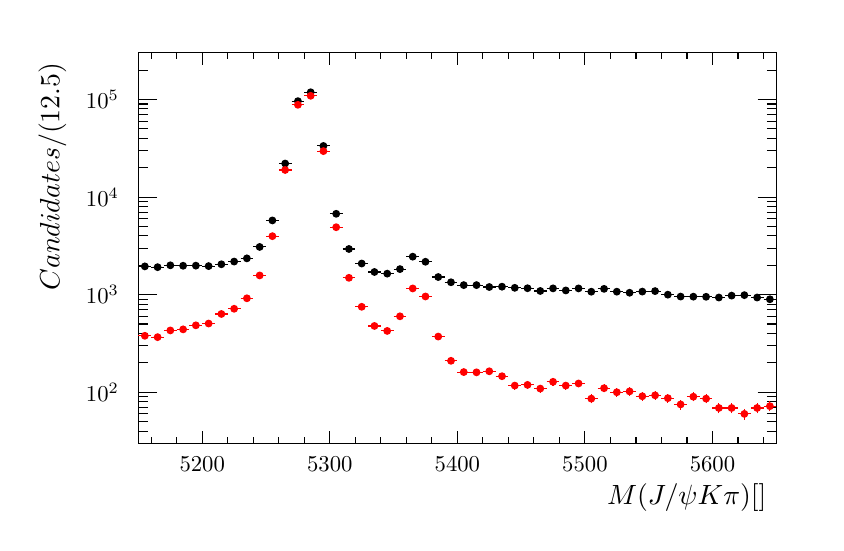
\begin{tikzpicture}
\pgfdeclareplotmark{cross} {
\pgfpathmoveto{\pgfpoint{-0.3\pgfplotmarksize}{\pgfplotmarksize}}
\pgfpathlineto{\pgfpoint{+0.3\pgfplotmarksize}{\pgfplotmarksize}}
\pgfpathlineto{\pgfpoint{+0.3\pgfplotmarksize}{0.3\pgfplotmarksize}}
\pgfpathlineto{\pgfpoint{+1\pgfplotmarksize}{0.3\pgfplotmarksize}}
\pgfpathlineto{\pgfpoint{+1\pgfplotmarksize}{-0.3\pgfplotmarksize}}
\pgfpathlineto{\pgfpoint{+0.3\pgfplotmarksize}{-0.3\pgfplotmarksize}}
\pgfpathlineto{\pgfpoint{+0.3\pgfplotmarksize}{-1.\pgfplotmarksize}}
\pgfpathlineto{\pgfpoint{-0.3\pgfplotmarksize}{-1.\pgfplotmarksize}}
\pgfpathlineto{\pgfpoint{-0.3\pgfplotmarksize}{-0.3\pgfplotmarksize}}
\pgfpathlineto{\pgfpoint{-1.\pgfplotmarksize}{-0.3\pgfplotmarksize}}
\pgfpathlineto{\pgfpoint{-1.\pgfplotmarksize}{0.3\pgfplotmarksize}}
\pgfpathlineto{\pgfpoint{-0.3\pgfplotmarksize}{0.3\pgfplotmarksize}}
\pgfpathclose
\pgfusepathqstroke
}
\pgfdeclareplotmark{cross*} {
\pgfpathmoveto{\pgfpoint{-0.3\pgfplotmarksize}{\pgfplotmarksize}}
\pgfpathlineto{\pgfpoint{+0.3\pgfplotmarksize}{\pgfplotmarksize}}
\pgfpathlineto{\pgfpoint{+0.3\pgfplotmarksize}{0.3\pgfplotmarksize}}
\pgfpathlineto{\pgfpoint{+1\pgfplotmarksize}{0.3\pgfplotmarksize}}
\pgfpathlineto{\pgfpoint{+1\pgfplotmarksize}{-0.3\pgfplotmarksize}}
\pgfpathlineto{\pgfpoint{+0.3\pgfplotmarksize}{-0.3\pgfplotmarksize}}
\pgfpathlineto{\pgfpoint{+0.3\pgfplotmarksize}{-1.\pgfplotmarksize}}
\pgfpathlineto{\pgfpoint{-0.3\pgfplotmarksize}{-1.\pgfplotmarksize}}
\pgfpathlineto{\pgfpoint{-0.3\pgfplotmarksize}{-0.3\pgfplotmarksize}}
\pgfpathlineto{\pgfpoint{-1.\pgfplotmarksize}{-0.3\pgfplotmarksize}}
\pgfpathlineto{\pgfpoint{-1.\pgfplotmarksize}{0.3\pgfplotmarksize}}
\pgfpathlineto{\pgfpoint{-0.3\pgfplotmarksize}{0.3\pgfplotmarksize}}
\pgfpathclose
\pgfusepathqfillstroke
}
\pgfdeclareplotmark{newstar} {
\pgfpathmoveto{\pgfqpoint{0pt}{\pgfplotmarksize}}
\pgfpathlineto{\pgfqpointpolar{44}{0.5\pgfplotmarksize}}
\pgfpathlineto{\pgfqpointpolar{18}{\pgfplotmarksize}}
\pgfpathlineto{\pgfqpointpolar{-20}{0.5\pgfplotmarksize}}
\pgfpathlineto{\pgfqpointpolar{-54}{\pgfplotmarksize}}
\pgfpathlineto{\pgfqpointpolar{-90}{0.5\pgfplotmarksize}}
\pgfpathlineto{\pgfqpointpolar{234}{\pgfplotmarksize}}
\pgfpathlineto{\pgfqpointpolar{198}{0.5\pgfplotmarksize}}
\pgfpathlineto{\pgfqpointpolar{162}{\pgfplotmarksize}}
\pgfpathlineto{\pgfqpointpolar{134}{0.5\pgfplotmarksize}}
\pgfpathclose
\pgfusepathqstroke
}
\pgfdeclareplotmark{newstar*} {
\pgfpathmoveto{\pgfqpoint{0pt}{\pgfplotmarksize}}
\pgfpathlineto{\pgfqpointpolar{44}{0.5\pgfplotmarksize}}
\pgfpathlineto{\pgfqpointpolar{18}{\pgfplotmarksize}}
\pgfpathlineto{\pgfqpointpolar{-20}{0.5\pgfplotmarksize}}
\pgfpathlineto{\pgfqpointpolar{-54}{\pgfplotmarksize}}
\pgfpathlineto{\pgfqpointpolar{-90}{0.5\pgfplotmarksize}}
\pgfpathlineto{\pgfqpointpolar{234}{\pgfplotmarksize}}
\pgfpathlineto{\pgfqpointpolar{198}{0.5\pgfplotmarksize}}
\pgfpathlineto{\pgfqpointpolar{162}{\pgfplotmarksize}}
\pgfpathlineto{\pgfqpointpolar{134}{0.5\pgfplotmarksize}}
\pgfpathclose
\pgfusepathqfillstroke
}
\definecolor{c}{rgb}{1,1,1};
\draw [color=c, fill=c] (0,0) rectangle (10,6.27517);
\draw [color=c, fill=c] (1.4,1.00403) rectangle (9.5,5.96141);
\definecolor{c}{rgb}{0,0,0};
\draw [c] (1.4,1.00403) -- (1.4,5.96141) -- (9.5,5.96141) -- (9.5,1.00403) -- (1.4,1.00403);
\draw [c,line width=0.4] (1.4,3.25058) -- (1.44744,3.25058);
\draw [c,line width=0.4] (1.51456,3.25058) -- (1.562,3.25058);
\foreach \P in {(1.481,3.25058)}{\draw[mark options={color=c,fill=c},mark size=1.201201pt,mark=*] plot coordinates {\P};}
\draw [c,line width=0.4] (1.562,3.24054) -- (1.60944,3.24054);
\draw [c,line width=0.4] (1.67656,3.24054) -- (1.724,3.24054);
\foreach \P in {(1.643,3.24054)}{\draw[mark options={color=c,fill=c},mark size=1.201201pt,mark=*] plot coordinates {\P};}
\draw [c,line width=0.4] (1.724,3.26421) -- (1.77144,3.26421);
\draw [c,line width=0.4] (1.83856,3.26421) -- (1.886,3.26421);
\foreach \P in {(1.805,3.26421)}{\draw[mark options={color=c,fill=c},mark size=1.201201pt,mark=*] plot coordinates {\P};}
\draw [c,line width=0.4] (1.886,3.25853) -- (1.93344,3.25853);
\draw [c,line width=0.4] (2.00056,3.25853) -- (2.048,3.25853);
\foreach \P in {(1.967,3.25853)}{\draw[mark options={color=c,fill=c},mark size=1.201201pt,mark=*] plot coordinates {\P};}
\draw [c,line width=0.4] (2.048,3.25989) -- (2.09544,3.25989);
\draw [c,line width=0.4] (2.16256,3.25989) -- (2.21,3.25989);
\foreach \P in {(2.129,3.25989)}{\draw[mark options={color=c,fill=c},mark size=1.201201pt,mark=*] plot coordinates {\P};}
\draw [c,line width=0.4] (2.21,3.25416) -- (2.25744,3.25416);
\draw [c,line width=0.4] (2.32456,3.25416) -- (2.372,3.25416);
\foreach \P in {(2.291,3.25416)}{\draw[mark options={color=c,fill=c},mark size=1.201201pt,mark=*] plot coordinates {\P};}
\draw [c,line width=0.4] (2.372,3.27725) -- (2.41944,3.27725);
\draw [c,line width=0.4] (2.48656,3.27725) -- (2.534,3.27725);
\foreach \P in {(2.453,3.27725)}{\draw[mark options={color=c,fill=c},mark size=1.201201pt,mark=*] plot coordinates {\P};}
\draw [c,line width=0.4] (2.534,3.3116) -- (2.58144,3.3116);
\draw [c,line width=0.4] (2.64856,3.3116) -- (2.696,3.3116);
\foreach \P in {(2.615,3.3116)}{\draw[mark options={color=c,fill=c},mark size=1.201201pt,mark=*] plot coordinates {\P};}
\draw [c,line width=0.4] (2.696,3.35243) -- (2.74344,3.35243);
\draw [c,line width=0.4] (2.81056,3.35243) -- (2.858,3.35243);
\foreach \P in {(2.777,3.35243)}{\draw[mark options={color=c,fill=c},mark size=1.201201pt,mark=*] plot coordinates {\P};}
\draw [c,line width=0.4] (2.858,3.49741) -- (2.90544,3.49741);
\draw [c,line width=0.4] (2.97256,3.49741) -- (3.02,3.49741);
\foreach \P in {(2.939,3.49741)}{\draw[mark options={color=c,fill=c},mark size=1.201201pt,mark=*] plot coordinates {\P};}
\draw [c,line width=0.4] (3.02,3.83411) -- (3.06744,3.83411);
\draw [c,line width=0.4] (3.13456,3.83411) -- (3.182,3.83411);
\foreach \P in {(3.101,3.83411)}{\draw[mark options={color=c,fill=c},mark size=1.201201pt,mark=*] plot coordinates {\P};}
\draw [c,line width=0.4] (3.182,4.55666) -- (3.22944,4.55666);
\draw [c,line width=0.4] (3.29656,4.55666) -- (3.344,4.55666);
\foreach \P in {(3.263,4.55666)}{\draw[mark options={color=c,fill=c},mark size=1.201201pt,mark=*] plot coordinates {\P};}
\draw [c,line width=0.4] (3.344,5.34895) -- (3.39144,5.34895);
\draw [c,line width=0.4] (3.45856,5.34895) -- (3.506,5.34895);
\foreach \P in {(3.425,5.34895)}{\draw[mark options={color=c,fill=c},mark size=1.201201pt,mark=*] plot coordinates {\P};}
\draw [c,line width=0.4] (3.506,5.46194) -- (3.55344,5.46194);
\draw [c,line width=0.4] (3.62056,5.46194) -- (3.668,5.46194);
\foreach \P in {(3.587,5.46194)}{\draw[mark options={color=c,fill=c},mark size=1.201201pt,mark=*] plot coordinates {\P};}
\draw [c,line width=0.4] (3.668,4.78019) -- (3.71544,4.78019);
\draw [c,line width=0.4] (3.78256,4.78019) -- (3.83,4.78019);
\foreach \P in {(3.749,4.78019)}{\draw[mark options={color=c,fill=c},mark size=1.201201pt,mark=*] plot coordinates {\P};}
\draw [c,line width=0.4] (3.83,3.9184) -- (3.87744,3.9184);
\draw [c,line width=0.4] (3.94456,3.9184) -- (3.992,3.9184);
\foreach \P in {(3.911,3.9184)}{\draw[mark options={color=c,fill=c},mark size=1.201201pt,mark=*] plot coordinates {\P};}
\draw [c,line width=0.4] (3.992,3.47166) -- (4.03944,3.47166);
\draw [c,line width=0.4] (4.10656,3.47166) -- (4.154,3.47166);
\foreach \P in {(4.073,3.47166)}{\draw[mark options={color=c,fill=c},mark size=1.201201pt,mark=*] plot coordinates {\P};}
\draw [c,line width=0.4] (4.154,3.28688) -- (4.20144,3.28688);
\draw [c,line width=0.4] (4.26856,3.28688) -- (4.316,3.28688);
\foreach \P in {(4.235,3.28688)}{\draw[mark options={color=c,fill=c},mark size=1.201201pt,mark=*] plot coordinates {\P};}
\draw [c,line width=0.4] (4.316,3.17953) -- (4.36344,3.17953);
\draw [c,line width=0.4] (4.43056,3.17953) -- (4.478,3.17953);
\foreach \P in {(4.397,3.17953)}{\draw[mark options={color=c,fill=c},mark size=1.201201pt,mark=*] plot coordinates {\P};}
\draw [c,line width=0.4] (4.478,3.15832) -- (4.52544,3.15832);
\draw [c,line width=0.4] (4.59256,3.15832) -- (4.64,3.15832);
\foreach \P in {(4.559,3.15832)}{\draw[mark options={color=c,fill=c},mark size=1.201201pt,mark=*] plot coordinates {\P};}
\draw [c,line width=0.4] (4.64,3.21608) -- (4.68744,3.21608);
\draw [c,line width=0.4] (4.75456,3.21608) -- (4.802,3.21608);
\foreach \P in {(4.721,3.21608)}{\draw[mark options={color=c,fill=c},mark size=1.201201pt,mark=*] plot coordinates {\P};}
\draw [c,line width=0.4] (4.802,3.37393) -- (4.84944,3.37393);
\draw [c,line width=0.4] (4.91656,3.37393) -- (4.964,3.37393);
\foreach \P in {(4.883,3.37393)}{\draw[mark options={color=c,fill=c},mark size=1.201201pt,mark=*] plot coordinates {\P};}
\draw [c,line width=0.4] (4.964,3.30938) -- (5.01144,3.30938);
\draw [c,line width=0.4] (5.07856,3.30938) -- (5.126,3.30938);
\foreach \P in {(5.045,3.30938)}{\draw[mark options={color=c,fill=c},mark size=1.201201pt,mark=*] plot coordinates {\P};}
\draw [c,line width=0.4] (5.126,3.11535) -- (5.17344,3.11535);
\draw [c,line width=0.4] (5.24056,3.11535) -- (5.288,3.11535);
\foreach \P in {(5.207,3.11535)}{\draw[mark options={color=c,fill=c},mark size=1.201201pt,mark=*] plot coordinates {\P};}
\draw [c,line width=0.4] (5.288,3.04893) -- (5.33544,3.04893);
\draw [c,line width=0.4] (5.40256,3.04893) -- (5.45,3.04893);
\foreach \P in {(5.369,3.04893)}{\draw[mark options={color=c,fill=c},mark size=1.201201pt,mark=*] plot coordinates {\P};}
\draw [c,line width=0.4] (5.45,3.0128) -- (5.49744,3.0128);
\draw [c,line width=0.4] (5.56456,3.0128) -- (5.612,3.0128);
\foreach \P in {(5.531,3.0128)}{\draw[mark options={color=c,fill=c},mark size=1.201201pt,mark=*] plot coordinates {\P};}
\draw [c,line width=0.4] (5.612,3.0128) -- (5.65944,3.0128);
\draw [c,line width=0.4] (5.72656,3.0128) -- (5.774,3.0128);
\foreach \P in {(5.693,3.0128)}{\draw[mark options={color=c,fill=c},mark size=1.201201pt,mark=*] plot coordinates {\P};}
\draw [c,line width=0.4] (5.774,2.98864) -- (5.82144,2.98864);
\draw [c,line width=0.4] (5.88856,2.98864) -- (5.936,2.98864);
\foreach \P in {(5.855,2.98864)}{\draw[mark options={color=c,fill=c},mark size=1.201201pt,mark=*] plot coordinates {\P};}
\draw [c,line width=0.4] (5.936,2.99266) -- (5.98344,2.99266);
\draw [c,line width=0.4] (6.05056,2.99266) -- (6.098,2.99266);
\foreach \P in {(6.017,2.99266)}{\draw[mark options={color=c,fill=c},mark size=1.201201pt,mark=*] plot coordinates {\P};}
\draw [c,line width=0.4] (6.098,2.9782) -- (6.14544,2.9782);
\draw [c,line width=0.4] (6.21256,2.9782) -- (6.26,2.9782);
\foreach \P in {(6.179,2.9782)}{\draw[mark options={color=c,fill=c},mark size=1.201201pt,mark=*] plot coordinates {\P};}
\draw [c,line width=0.4] (6.26,2.97314) -- (6.30744,2.97314);
\draw [c,line width=0.4] (6.37456,2.97314) -- (6.422,2.97314);
\foreach \P in {(6.341,2.97314)}{\draw[mark options={color=c,fill=c},mark size=1.201201pt,mark=*] plot coordinates {\P};}
\draw [c,line width=0.4] (6.422,2.93828) -- (6.46944,2.93828);
\draw [c,line width=0.4] (6.53656,2.93828) -- (6.584,2.93828);
\foreach \P in {(6.503,2.93828)}{\draw[mark options={color=c,fill=c},mark size=1.201201pt,mark=*] plot coordinates {\P};}
\draw [c,line width=0.4] (6.584,2.97129) -- (6.63144,2.97129);
\draw [c,line width=0.4] (6.69856,2.97129) -- (6.746,2.97129);
\foreach \P in {(6.665,2.97129)}{\draw[mark options={color=c,fill=c},mark size=1.201201pt,mark=*] plot coordinates {\P};}
\draw [c,line width=0.4] (6.746,2.94514) -- (6.79344,2.94514);
\draw [c,line width=0.4] (6.86056,2.94514) -- (6.908,2.94514);
\foreach \P in {(6.827,2.94514)}{\draw[mark options={color=c,fill=c},mark size=1.201201pt,mark=*] plot coordinates {\P};}
\draw [c,line width=0.4] (6.908,2.97082) -- (6.95544,2.97082);
\draw [c,line width=0.4] (7.02256,2.97082) -- (7.07,2.97082);
\foreach \P in {(6.989,2.97082)}{\draw[mark options={color=c,fill=c},mark size=1.201201pt,mark=*] plot coordinates {\P};}
\draw [c,line width=0.4] (7.07,2.92882) -- (7.11744,2.92882);
\draw [c,line width=0.4] (7.18456,2.92882) -- (7.232,2.92882);
\foreach \P in {(7.151,2.92882)}{\draw[mark options={color=c,fill=c},mark size=1.201201pt,mark=*] plot coordinates {\P};}
\draw [c,line width=0.4] (7.232,2.96522) -- (7.27944,2.96522);
\draw [c,line width=0.4] (7.34656,2.96522) -- (7.394,2.96522);
\foreach \P in {(7.313,2.96522)}{\draw[mark options={color=c,fill=c},mark size=1.201201pt,mark=*] plot coordinates {\P};}
\draw [c,line width=0.4] (7.394,2.92932) -- (7.44144,2.92932);
\draw [c,line width=0.4] (7.50856,2.92932) -- (7.556,2.92932);
\foreach \P in {(7.475,2.92932)}{\draw[mark options={color=c,fill=c},mark size=1.201201pt,mark=*] plot coordinates {\P};}
\draw [c,line width=0.4] (7.556,2.91561) -- (7.60344,2.91561);
\draw [c,line width=0.4] (7.67056,2.91561) -- (7.718,2.91561);
\foreach \P in {(7.637,2.91561)}{\draw[mark options={color=c,fill=c},mark size=1.201201pt,mark=*] plot coordinates {\P};}
\draw [c,line width=0.4] (7.718,2.93033) -- (7.76544,2.93033);
\draw [c,line width=0.4] (7.83256,2.93033) -- (7.88,2.93033);
\foreach \P in {(7.799,2.93033)}{\draw[mark options={color=c,fill=c},mark size=1.201201pt,mark=*] plot coordinates {\P};}
\draw [c,line width=0.4] (7.88,2.9368) -- (7.92744,2.9368);
\draw [c,line width=0.4] (7.99456,2.9368) -- (8.042,2.9368);
\foreach \P in {(7.961,2.9368)}{\draw[mark options={color=c,fill=c},mark size=1.201201pt,mark=*] plot coordinates {\P};}
\draw [c,line width=0.4] (8.042,2.8914) -- (8.08944,2.8914);
\draw [c,line width=0.4] (8.15656,2.8914) -- (8.204,2.8914);
\foreach \P in {(8.123,2.8914)}{\draw[mark options={color=c,fill=c},mark size=1.201201pt,mark=*] plot coordinates {\P};}
\draw [c,line width=0.4] (8.204,2.86718) -- (8.25144,2.86718);
\draw [c,line width=0.4] (8.31856,2.86718) -- (8.366,2.86718);
\foreach \P in {(8.285,2.86718)}{\draw[mark options={color=c,fill=c},mark size=1.201201pt,mark=*] plot coordinates {\P};}
\draw [c,line width=0.4] (8.366,2.86605) -- (8.41344,2.86605);
\draw [c,line width=0.4] (8.48056,2.86605) -- (8.528,2.86605);
\foreach \P in {(8.447,2.86605)}{\draw[mark options={color=c,fill=c},mark size=1.201201pt,mark=*] plot coordinates {\P};}
\draw [c,line width=0.4] (8.528,2.86436) -- (8.57544,2.86436);
\draw [c,line width=0.4] (8.64256,2.86436) -- (8.69,2.86436);
\foreach \P in {(8.609,2.86436)}{\draw[mark options={color=c,fill=c},mark size=1.201201pt,mark=*] plot coordinates {\P};}
\draw [c,line width=0.4] (8.69,2.85523) -- (8.73744,2.85523);
\draw [c,line width=0.4] (8.80456,2.85523) -- (8.852,2.85523);
\foreach \P in {(8.771,2.85523)}{\draw[mark options={color=c,fill=c},mark size=1.201201pt,mark=*] plot coordinates {\P};}
\draw [c,line width=0.4] (8.852,2.87943) -- (8.89944,2.87943);
\draw [c,line width=0.4] (8.96656,2.87943) -- (9.014,2.87943);
\foreach \P in {(8.933,2.87943)}{\draw[mark options={color=c,fill=c},mark size=1.201201pt,mark=*] plot coordinates {\P};}
\draw [c,line width=0.4] (9.014,2.88545) -- (9.06144,2.88545);
\draw [c,line width=0.4] (9.12856,2.88545) -- (9.176,2.88545);
\foreach \P in {(9.095,2.88545)}{\draw[mark options={color=c,fill=c},mark size=1.201201pt,mark=*] plot coordinates {\P};}
\draw [c,line width=0.4] (9.176,2.85523) -- (9.22344,2.85523);
\draw [c,line width=0.4] (9.29056,2.85523) -- (9.338,2.85523);
\foreach \P in {(9.257,2.85523)}{\draw[mark options={color=c,fill=c},mark size=1.201201pt,mark=*] plot coordinates {\P};}
\draw [c,line width=0.4] (9.338,2.83289) -- (9.38544,2.83289);
\draw [c,line width=0.4] (9.45256,2.83289) -- (9.5,2.83289);
\foreach \P in {(9.419,2.83289)}{\draw[mark options={color=c,fill=c},mark size=1.201201pt,mark=*] plot coordinates {\P};}
\draw [c,line width=0.4] (1.4,1.00403) -- (9.5,1.00403);
\draw [anchor= east] (9.5,0.317272) node[scale=1.00614, rotate=0]{$\text{M}(J/\psi K\pi)  [\mevcc]$};
\draw [c,line width=0.4] (2.21,1.15651) -- (2.21,1.00403);
\draw [c,line width=0.4] (2.534,1.08027) -- (2.534,1.00403);
\draw [c,line width=0.4] (2.858,1.08027) -- (2.858,1.00403);
\draw [c,line width=0.4] (3.182,1.08027) -- (3.182,1.00403);
\draw [c,line width=0.4] (3.506,1.08027) -- (3.506,1.00403);
\draw [c,line width=0.4] (3.83,1.15651) -- (3.83,1.00403);
\draw [c,line width=0.4] (4.154,1.08027) -- (4.154,1.00403);
\draw [c,line width=0.4] (4.478,1.08027) -- (4.478,1.00403);
\draw [c,line width=0.4] (4.802,1.08027) -- (4.802,1.00403);
\draw [c,line width=0.4] (5.126,1.08027) -- (5.126,1.00403);
\draw [c,line width=0.4] (5.45,1.15651) -- (5.45,1.00403);
\draw [c,line width=0.4] (5.774,1.08027) -- (5.774,1.00403);
\draw [c,line width=0.4] (6.098,1.08027) -- (6.098,1.00403);
\draw [c,line width=0.4] (6.422,1.08027) -- (6.422,1.00403);
\draw [c,line width=0.4] (6.746,1.08027) -- (6.746,1.00403);
\draw [c,line width=0.4] (7.07,1.15651) -- (7.07,1.00403);
\draw [c,line width=0.4] (7.394,1.08027) -- (7.394,1.00403);
\draw [c,line width=0.4] (7.718,1.08027) -- (7.718,1.00403);
\draw [c,line width=0.4] (8.042,1.08027) -- (8.042,1.00403);
\draw [c,line width=0.4] (8.366,1.08027) -- (8.366,1.00403);
\draw [c,line width=0.4] (8.69,1.15651) -- (8.69,1.00403);
\draw [c,line width=0.4] (2.21,1.15651) -- (2.21,1.00403);
\draw [c,line width=0.4] (1.886,1.08027) -- (1.886,1.00403);
\draw [c,line width=0.4] (1.562,1.08027) -- (1.562,1.00403);
\draw [c,line width=0.4] (8.69,1.15651) -- (8.69,1.00403);
\draw [c,line width=0.4] (9.014,1.08027) -- (9.014,1.00403);
\draw [c,line width=0.4] (9.338,1.08027) -- (9.338,1.00403);
\draw [anchor=base] (2.21,0.640067) node[scale=0.819821, rotate=0]{5200};
\draw [anchor=base] (3.83,0.640067) node[scale=0.819821, rotate=0]{5300};
\draw [anchor=base] (5.45,0.640067) node[scale=0.819821, rotate=0]{5400};
\draw [anchor=base] (7.07,0.640067) node[scale=0.819821, rotate=0]{5500};
\draw [anchor=base] (8.69,0.640067) node[scale=0.819821, rotate=0]{5600};
\draw [c,line width=0.4] (1.4,5.96141) -- (9.5,5.96141);
\draw [c,line width=0.4] (2.21,5.80892) -- (2.21,5.96141);
\draw [c,line width=0.4] (2.534,5.88517) -- (2.534,5.96141);
\draw [c,line width=0.4] (2.858,5.88517) -- (2.858,5.96141);
\draw [c,line width=0.4] (3.182,5.88517) -- (3.182,5.96141);
\draw [c,line width=0.4] (3.506,5.88517) -- (3.506,5.96141);
\draw [c,line width=0.4] (3.83,5.80892) -- (3.83,5.96141);
\draw [c,line width=0.4] (4.154,5.88517) -- (4.154,5.96141);
\draw [c,line width=0.4] (4.478,5.88517) -- (4.478,5.96141);
\draw [c,line width=0.4] (4.802,5.88517) -- (4.802,5.96141);
\draw [c,line width=0.4] (5.126,5.88517) -- (5.126,5.96141);
\draw [c,line width=0.4] (5.45,5.80892) -- (5.45,5.96141);
\draw [c,line width=0.4] (5.774,5.88517) -- (5.774,5.96141);
\draw [c,line width=0.4] (6.098,5.88517) -- (6.098,5.96141);
\draw [c,line width=0.4] (6.422,5.88517) -- (6.422,5.96141);
\draw [c,line width=0.4] (6.746,5.88517) -- (6.746,5.96141);
\draw [c,line width=0.4] (7.07,5.80892) -- (7.07,5.96141);
\draw [c,line width=0.4] (7.394,5.88517) -- (7.394,5.96141);
\draw [c,line width=0.4] (7.718,5.88517) -- (7.718,5.96141);
\draw [c,line width=0.4] (8.042,5.88517) -- (8.042,5.96141);
\draw [c,line width=0.4] (8.366,5.88517) -- (8.366,5.96141);
\draw [c,line width=0.4] (8.69,5.80892) -- (8.69,5.96141);
\draw [c,line width=0.4] (2.21,5.80892) -- (2.21,5.96141);
\draw [c,line width=0.4] (1.886,5.88517) -- (1.886,5.96141);
\draw [c,line width=0.4] (1.562,5.88517) -- (1.562,5.96141);
\draw [c,line width=0.4] (8.69,5.80892) -- (8.69,5.96141);
\draw [c,line width=0.4] (9.014,5.88517) -- (9.014,5.96141);
\draw [c,line width=0.4] (9.338,5.88517) -- (9.338,5.96141);
\draw [c,line width=0.4] (1.4,1.00403) -- (1.4,5.96141);
\draw [anchor= east] (0.3056,5.96141) node[scale=1.00614, rotate=90]{$\text{Candidates} / (12.5 \mevcc)$};
\draw [c,line width=0.4] (1.5185,1.15887) -- (1.4,1.15887);
\draw [c,line width=0.4] (1.5185,1.27897) -- (1.4,1.27897);
\draw [c,line width=0.4] (1.5185,1.37711) -- (1.4,1.37711);
\draw [c,line width=0.4] (1.5185,1.46008) -- (1.4,1.46008);
\draw [c,line width=0.4] (1.5185,1.53195) -- (1.4,1.53195);
\draw [c,line width=0.4] (1.5185,1.59534) -- (1.4,1.59534);
\draw [c,line width=0.4] (1.637,1.65205) -- (1.4,1.65205);
\draw [anchor= east] (1.252,1.65205) node[scale=0.819821, rotate=0]{$10^{2}$};
\draw [c,line width=0.4] (1.5185,2.02513) -- (1.4,2.02513);
\draw [c,line width=0.4] (1.5185,2.24337) -- (1.4,2.24337);
\draw [c,line width=0.4] (1.5185,2.39821) -- (1.4,2.39821);
\draw [c,line width=0.4] (1.5185,2.51832) -- (1.4,2.51832);
\draw [c,line width=0.4] (1.5185,2.61645) -- (1.4,2.61645);
\draw [c,line width=0.4] (1.5185,2.69942) -- (1.4,2.69942);
\draw [c,line width=0.4] (1.5185,2.77129) -- (1.4,2.77129);
\draw [c,line width=0.4] (1.5185,2.83469) -- (1.4,2.83469);
\draw [c,line width=0.4] (1.637,2.8914) -- (1.4,2.8914);
\draw [anchor= east] (1.252,2.8914) node[scale=0.819821, rotate=0]{$10^{3}$};
\draw [c,line width=0.4] (1.5185,3.26448) -- (1.4,3.26448);
\draw [c,line width=0.4] (1.5185,3.48272) -- (1.4,3.48272);
\draw [c,line width=0.4] (1.5185,3.63756) -- (1.4,3.63756);
\draw [c,line width=0.4] (1.5185,3.75766) -- (1.4,3.75766);
\draw [c,line width=0.4] (1.5185,3.8558) -- (1.4,3.8558);
\draw [c,line width=0.4] (1.5185,3.93877) -- (1.4,3.93877);
\draw [c,line width=0.4] (1.5185,4.01064) -- (1.4,4.01064);
\draw [c,line width=0.4] (1.5185,4.07404) -- (1.4,4.07404);
\draw [c,line width=0.4] (1.637,4.13075) -- (1.4,4.13075);
\draw [anchor= east] (1.252,4.13075) node[scale=0.819821, rotate=0]{$10^{4}$};
\draw [c,line width=0.4] (1.5185,4.50383) -- (1.4,4.50383);
\draw [c,line width=0.4] (1.5185,4.72206) -- (1.4,4.72206);
\draw [c,line width=0.4] (1.5185,4.87691) -- (1.4,4.87691);
\draw [c,line width=0.4] (1.5185,4.99701) -- (1.4,4.99701);
\draw [c,line width=0.4] (1.5185,5.09514) -- (1.4,5.09514);
\draw [c,line width=0.4] (1.5185,5.17811) -- (1.4,5.17811);
\draw [c,line width=0.4] (1.5185,5.24999) -- (1.4,5.24999);
\draw [c,line width=0.4] (1.5185,5.31338) -- (1.4,5.31338);
\draw [c,line width=0.4] (1.637,5.37009) -- (1.4,5.37009);
\draw [anchor= east] (1.252,5.37009) node[scale=0.819821, rotate=0]{$10^{5}$};
\draw [c,line width=0.4] (1.5185,5.74317) -- (1.4,5.74317);
\draw [c,line width=0.4] (1.5185,5.96141) -- (1.4,5.96141);
\draw [c,line width=0.4] (9.5,1.00403) -- (9.5,5.96141);
\draw [c,line width=0.4] (9.3815,1.15887) -- (9.5,1.15887);
\draw [c,line width=0.4] (9.3815,1.27897) -- (9.5,1.27897);
\draw [c,line width=0.4] (9.3815,1.37711) -- (9.5,1.37711);
\draw [c,line width=0.4] (9.3815,1.46008) -- (9.5,1.46008);
\draw [c,line width=0.4] (9.3815,1.53195) -- (9.5,1.53195);
\draw [c,line width=0.4] (9.3815,1.59534) -- (9.5,1.59534);
\draw [c,line width=0.4] (9.263,1.65205) -- (9.5,1.65205);
\draw [c,line width=0.4] (9.3815,2.02513) -- (9.5,2.02513);
\draw [c,line width=0.4] (9.3815,2.24337) -- (9.5,2.24337);
\draw [c,line width=0.4] (9.3815,2.39821) -- (9.5,2.39821);
\draw [c,line width=0.4] (9.3815,2.51832) -- (9.5,2.51832);
\draw [c,line width=0.4] (9.3815,2.61645) -- (9.5,2.61645);
\draw [c,line width=0.4] (9.3815,2.69942) -- (9.5,2.69942);
\draw [c,line width=0.4] (9.3815,2.77129) -- (9.5,2.77129);
\draw [c,line width=0.4] (9.3815,2.83469) -- (9.5,2.83469);
\draw [c,line width=0.4] (9.263,2.8914) -- (9.5,2.8914);
\draw [c,line width=0.4] (9.3815,3.26448) -- (9.5,3.26448);
\draw [c,line width=0.4] (9.3815,3.48272) -- (9.5,3.48272);
\draw [c,line width=0.4] (9.3815,3.63756) -- (9.5,3.63756);
\draw [c,line width=0.4] (9.3815,3.75766) -- (9.5,3.75766);
\draw [c,line width=0.4] (9.3815,3.8558) -- (9.5,3.8558);
\draw [c,line width=0.4] (9.3815,3.93877) -- (9.5,3.93877);
\draw [c,line width=0.4] (9.3815,4.01064) -- (9.5,4.01064);
\draw [c,line width=0.4] (9.3815,4.07404) -- (9.5,4.07404);
\draw [c,line width=0.4] (9.263,4.13075) -- (9.5,4.13075);
\draw [c,line width=0.4] (9.3815,4.50383) -- (9.5,4.50383);
\draw [c,line width=0.4] (9.3815,4.72206) -- (9.5,4.72206);
\draw [c,line width=0.4] (9.3815,4.87691) -- (9.5,4.87691);
\draw [c,line width=0.4] (9.3815,4.99701) -- (9.5,4.99701);
\draw [c,line width=0.4] (9.3815,5.09514) -- (9.5,5.09514);
\draw [c,line width=0.4] (9.3815,5.17811) -- (9.5,5.17811);
\draw [c,line width=0.4] (9.3815,5.24999) -- (9.5,5.24999);
\draw [c,line width=0.4] (9.3815,5.31338) -- (9.5,5.31338);
\draw [c,line width=0.4] (9.263,5.37009) -- (9.5,5.37009);
\draw [c,line width=0.4] (9.3815,5.74317) -- (9.5,5.74317);
\draw [c,line width=0.4] (9.3815,5.96141) -- (9.5,5.96141);
\definecolor{c}{rgb}{1,0,0};
\draw [c,line width=0.4] (1.4,2.36919) -- (1.44744,2.36919);
\draw [c,line width=0.4] (1.51456,2.36919) -- (1.562,2.36919);
\foreach \P in {(1.481,2.36919)}{\draw[mark options={color=c,fill=c},mark size=1.201201pt,mark=*] plot coordinates {\P};}
\draw [c,line width=0.4] (1.562,2.35187) -- (1.60944,2.35187);
\draw [c,line width=0.4] (1.67656,2.35187) -- (1.724,2.35187);
\foreach \P in {(1.643,2.35187)}{\draw[mark options={color=c,fill=c},mark size=1.201201pt,mark=*] plot coordinates {\P};}
\draw [c,line width=0.4] (1.724,2.43714) -- (1.77144,2.43714);
\draw [c,line width=0.4] (1.83856,2.43714) -- (1.886,2.43714);
\foreach \P in {(1.805,2.43714)}{\draw[mark options={color=c,fill=c},mark size=1.201201pt,mark=*] plot coordinates {\P};}
\draw [c,line width=0.4] (1.886,2.45074) -- (1.93344,2.45074);
\draw [c,line width=0.4] (2.00056,2.45074) -- (2.048,2.45074);
\foreach \P in {(1.967,2.45074)}{\draw[mark options={color=c,fill=c},mark size=1.201201pt,mark=*] plot coordinates {\P};}
\draw [c,line width=0.4] (2.048,2.50193) -- (2.09544,2.50193);
\draw [c,line width=0.4] (2.16256,2.50193) -- (2.21,2.50193);
\foreach \P in {(2.129,2.50193)}{\draw[mark options={color=c,fill=c},mark size=1.201201pt,mark=*] plot coordinates {\P};}
\draw [c,line width=0.4] (2.21,2.52474) -- (2.25744,2.52474);
\draw [c,line width=0.4] (2.32456,2.52474) -- (2.372,2.52474);
\foreach \P in {(2.291,2.52474)}{\draw[mark options={color=c,fill=c},mark size=1.201201pt,mark=*] plot coordinates {\P};}
\draw [c,line width=0.4] (2.372,2.64612) -- (2.41944,2.64612);
\draw [c,line width=0.4] (2.48656,2.64612) -- (2.534,2.64612);
\foreach \P in {(2.453,2.64612)}{\draw[mark options={color=c,fill=c},mark size=1.201201pt,mark=*] plot coordinates {\P};}
\draw [c,line width=0.4] (2.534,2.71234) -- (2.58144,2.71234);
\draw [c,line width=0.4] (2.64856,2.71234) -- (2.696,2.71234);
\foreach \P in {(2.615,2.71234)}{\draw[mark options={color=c,fill=c},mark size=1.201201pt,mark=*] plot coordinates {\P};}
\draw [c,line width=0.4] (2.696,2.84535) -- (2.74344,2.84535);
\draw [c,line width=0.4] (2.81056,2.84535) -- (2.858,2.84535);
\foreach \P in {(2.777,2.84535)}{\draw[mark options={color=c,fill=c},mark size=1.201201pt,mark=*] plot coordinates {\P};}
\draw [c,line width=0.4] (2.858,3.13556) -- (2.90544,3.13556);
\draw [c,line width=0.4] (2.97256,3.13556) -- (3.02,3.13556);
\foreach \P in {(2.939,3.13556)}{\draw[mark options={color=c,fill=c},mark size=1.201201pt,mark=*] plot coordinates {\P};}
\draw [c,line width=0.4] (3.02,3.63432) -- (3.06744,3.63432);
\draw [c,line width=0.4] (3.13456,3.63432) -- (3.182,3.63432);
\foreach \P in {(3.101,3.63432)}{\draw[mark options={color=c,fill=c},mark size=1.201201pt,mark=*] plot coordinates {\P};}
\draw [c,line width=0.4] (3.182,4.47494) -- (3.22944,4.47494);
\draw [c,line width=0.4] (3.29656,4.47494) -- (3.344,4.47494);
\foreach \P in {(3.263,4.47494)}{\draw[mark options={color=c,fill=c},mark size=1.201201pt,mark=*] plot coordinates {\P};}
\draw [c,line width=0.4] (3.344,5.30249) -- (3.39144,5.30249);
\draw [c,line width=0.4] (3.45856,5.30249) -- (3.506,5.30249);
\foreach \P in {(3.425,5.30249)}{\draw[mark options={color=c,fill=c},mark size=1.201201pt,mark=*] plot coordinates {\P};}
\draw [c,line width=0.4] (3.506,5.4168) -- (3.55344,5.4168);
\draw [c,line width=0.4] (3.62056,5.4168) -- (3.668,5.4168);
\foreach \P in {(3.587,5.4168)}{\draw[mark options={color=c,fill=c},mark size=1.201201pt,mark=*] plot coordinates {\P};}
\draw [c,line width=0.4] (3.668,4.71451) -- (3.71544,4.71451);
\draw [c,line width=0.4] (3.78256,4.71451) -- (3.83,4.71451);
\foreach \P in {(3.749,4.71451)}{\draw[mark options={color=c,fill=c},mark size=1.201201pt,mark=*] plot coordinates {\P};}
\draw [c,line width=0.4] (3.83,3.748) -- (3.87744,3.748);
\draw [c,line width=0.4] (3.94456,3.748) -- (3.992,3.748);
\foreach \P in {(3.911,3.748)}{\draw[mark options={color=c,fill=c},mark size=1.201201pt,mark=*] plot coordinates {\P};}
\draw [c,line width=0.4] (3.992,3.10531) -- (4.03944,3.10531);
\draw [c,line width=0.4] (4.10656,3.10531) -- (4.154,3.10531);
\foreach \P in {(4.073,3.10531)}{\draw[mark options={color=c,fill=c},mark size=1.201201pt,mark=*] plot coordinates {\P};}
\draw [c,line width=0.4] (4.154,2.73727) -- (4.20144,2.73727);
\draw [c,line width=0.4] (4.26856,2.73727) -- (4.316,2.73727);
\foreach \P in {(4.235,2.73727)}{\draw[mark options={color=c,fill=c},mark size=1.201201pt,mark=*] plot coordinates {\P};}
\draw [c,line width=0.4] (4.316,2.4941) -- (4.36344,2.4941);
\draw [c,line width=0.4] (4.43056,2.4941) -- (4.478,2.4941);
\foreach \P in {(4.397,2.4941)}{\draw[mark options={color=c,fill=c},mark size=1.201201pt,mark=*] plot coordinates {\P};}
\draw [c,line width=0.4] (4.478,2.43085) -- (4.52544,2.43085);
\draw [c,line width=0.4] (4.59256,2.43085) -- (4.64,2.43085);
\foreach \P in {(4.559,2.43085)}{\draw[mark options={color=c,fill=c},mark size=1.201201pt,mark=*] plot coordinates {\P};}
\draw [c,line width=0.4] (4.64,2.61645) -- (4.68744,2.61645);
\draw [c,line width=0.4] (4.75456,2.61645) -- (4.802,2.61645);
\foreach \P in {(4.721,2.61645)}{\draw[mark options={color=c,fill=c},mark size=1.201201pt,mark=*] plot coordinates {\P};}
\draw [c,line width=0.4] (4.802,2.97036) -- (4.84944,2.97036);
\draw [c,line width=0.4] (4.91656,2.97036) -- (4.964,2.97036);
\foreach \P in {(4.883,2.97036)}{\draw[mark options={color=c,fill=c},mark size=1.201201pt,mark=*] plot coordinates {\P};}
\draw [c,line width=0.4] (4.964,2.86831) -- (5.01144,2.86831);
\draw [c,line width=0.4] (5.07856,2.86831) -- (5.126,2.86831);
\foreach \P in {(5.045,2.86831)}{\draw[mark options={color=c,fill=c},mark size=1.201201pt,mark=*] plot coordinates {\P};}
\draw [c,line width=0.4] (5.126,2.35915) -- (5.17344,2.35915);
\draw [c,line width=0.4] (5.24056,2.35915) -- (5.288,2.35915);
\foreach \P in {(5.207,2.35915)}{\draw[mark options={color=c,fill=c},mark size=1.201201pt,mark=*] plot coordinates {\P};}
\draw [c,line width=0.4] (5.369,2.01291) -- (5.369,2.01784);
\draw [c,line width=0.4] (5.369,2.08495) -- (5.369,2.08731);
\draw [c,line width=0.4] (5.288,2.0514) -- (5.33544,2.0514);
\draw [c,line width=0.4] (5.40256,2.0514) -- (5.45,2.0514);
\foreach \P in {(5.369,2.0514)}{\draw[mark options={color=c,fill=c},mark size=1.201201pt,mark=*] plot coordinates {\P};}
\draw [c,line width=0.4] (5.531,1.8642) -- (5.531,1.87483);
\draw [c,line width=0.4] (5.531,1.94194) -- (5.531,1.94921);
\draw [c,line width=0.4] (5.45,1.90838) -- (5.49744,1.90838);
\draw [c,line width=0.4] (5.56456,1.90838) -- (5.612,1.90838);
\foreach \P in {(5.531,1.90838)}{\draw[mark options={color=c,fill=c},mark size=1.201201pt,mark=*] plot coordinates {\P};}
\draw [c,line width=0.4] (5.693,1.8607) -- (5.693,1.87147);
\draw [c,line width=0.4] (5.693,1.93859) -- (5.693,1.94598);
\draw [c,line width=0.4] (5.612,1.90503) -- (5.65944,1.90503);
\draw [c,line width=0.4] (5.72656,1.90503) -- (5.774,1.90503);
\foreach \P in {(5.693,1.90503)}{\draw[mark options={color=c,fill=c},mark size=1.201201pt,mark=*] plot coordinates {\P};}
\draw [c,line width=0.4] (5.855,1.87456) -- (5.855,1.88476);
\draw [c,line width=0.4] (5.855,1.95188) -- (5.855,1.95879);
\draw [c,line width=0.4] (5.774,1.91832) -- (5.82144,1.91832);
\draw [c,line width=0.4] (5.88856,1.91832) -- (5.936,1.91832);
\foreach \P in {(5.855,1.91832)}{\draw[mark options={color=c,fill=c},mark size=1.201201pt,mark=*] plot coordinates {\P};}
\draw [c,line width=0.4] (6.017,1.80925) -- (6.017,1.82219);
\draw [c,line width=0.4] (6.017,1.8893) -- (6.017,1.89854);
\draw [c,line width=0.4] (5.936,1.85574) -- (5.98344,1.85574);
\draw [c,line width=0.4] (6.05056,1.85574) -- (6.098,1.85574);
\foreach \P in {(6.017,1.85574)}{\draw[mark options={color=c,fill=c},mark size=1.201201pt,mark=*] plot coordinates {\P};}
\draw [c,line width=0.4] (6.179,1.68435) -- (6.179,1.703);
\draw [c,line width=0.4] (6.179,1.77012) -- (6.179,1.78415);
\draw [c,line width=0.4] (6.098,1.73656) -- (6.14544,1.73656);
\draw [c,line width=0.4] (6.21256,1.73656) -- (6.26,1.73656);
\foreach \P in {(6.179,1.73656)}{\draw[mark options={color=c,fill=c},mark size=1.201201pt,mark=*] plot coordinates {\P};}
\draw [c,line width=0.4] (6.341,1.69393) -- (6.341,1.71213);
\draw [c,line width=0.4] (6.341,1.77924) -- (6.341,1.79289);
\draw [c,line width=0.4] (6.26,1.74568) -- (6.30744,1.74568);
\draw [c,line width=0.4] (6.37456,1.74568) -- (6.422,1.74568);
\foreach \P in {(6.341,1.74568)}{\draw[mark options={color=c,fill=c},mark size=1.201201pt,mark=*] plot coordinates {\P};}
\draw [c,line width=0.4] (6.503,1.64425) -- (6.503,1.66488);
\draw [c,line width=0.4] (6.503,1.732) -- (6.503,1.74767);
\draw [c,line width=0.4] (6.422,1.69844) -- (6.46944,1.69844);
\draw [c,line width=0.4] (6.53656,1.69844) -- (6.584,1.69844);
\foreach \P in {(6.503,1.69844)}{\draw[mark options={color=c,fill=c},mark size=1.201201pt,mark=*] plot coordinates {\P};}
\draw [c,line width=0.4] (6.665,1.73512) -- (6.665,1.75137);
\draw [c,line width=0.4] (6.665,1.81848) -- (6.665,1.83051);
\draw [c,line width=0.4] (6.584,1.78492) -- (6.63144,1.78492);
\draw [c,line width=0.4] (6.69856,1.78492) -- (6.746,1.78492);
\foreach \P in {(6.665,1.78492)}{\draw[mark options={color=c,fill=c},mark size=1.201201pt,mark=*] plot coordinates {\P};}
\draw [c,line width=0.4] (6.827,1.68435) -- (6.827,1.703);
\draw [c,line width=0.4] (6.827,1.77012) -- (6.827,1.78415);
\draw [c,line width=0.4] (6.746,1.73656) -- (6.79344,1.73656);
\draw [c,line width=0.4] (6.86056,1.73656) -- (6.908,1.73656);
\foreach \P in {(6.827,1.73656)}{\draw[mark options={color=c,fill=c},mark size=1.201201pt,mark=*] plot coordinates {\P};}
\draw [c,line width=0.4] (6.989,1.71262) -- (6.989,1.72992);
\draw [c,line width=0.4] (6.989,1.79703) -- (6.989,1.80994);
\draw [c,line width=0.4] (6.908,1.76348) -- (6.95544,1.76348);
\draw [c,line width=0.4] (7.02256,1.76348) -- (7.07,1.76348);
\foreach \P in {(6.989,1.76348)}{\draw[mark options={color=c,fill=c},mark size=1.201201pt,mark=*] plot coordinates {\P};}
\draw [c,line width=0.4] (7.151,1.50946) -- (7.151,1.53732);
\draw [c,line width=0.4] (7.151,1.60443) -- (7.151,1.62599);
\draw [c,line width=0.4] (7.07,1.57088) -- (7.11744,1.57088);
\draw [c,line width=0.4] (7.18456,1.57088) -- (7.232,1.57088);
\foreach \P in {(7.151,1.57088)}{\draw[mark options={color=c,fill=c},mark size=1.201201pt,mark=*] plot coordinates {\P};}
\draw [c,line width=0.4] (7.313,1.64942) -- (7.313,1.6698);
\draw [c,line width=0.4] (7.313,1.73691) -- (7.313,1.75237);
\draw [c,line width=0.4] (7.232,1.70335) -- (7.27944,1.70335);
\draw [c,line width=0.4] (7.34656,1.70335) -- (7.394,1.70335);
\foreach \P in {(7.313,1.70335)}{\draw[mark options={color=c,fill=c},mark size=1.201201pt,mark=*] plot coordinates {\P};}
\draw [c,line width=0.4] (7.475,1.59535) -- (7.475,1.6185);
\draw [c,line width=0.4] (7.475,1.68561) -- (7.475,1.70335);
\draw [c,line width=0.4] (7.394,1.65205) -- (7.44144,1.65205);
\draw [c,line width=0.4] (7.50856,1.65205) -- (7.556,1.65205);
\foreach \P in {(7.475,1.65205)}{\draw[mark options={color=c,fill=c},mark size=1.201201pt,mark=*] plot coordinates {\P};}
\draw [c,line width=0.4] (7.637,1.60659) -- (7.637,1.62916);
\draw [c,line width=0.4] (7.637,1.69627) -- (7.637,1.71353);
\draw [c,line width=0.4] (7.556,1.66271) -- (7.60344,1.66271);
\draw [c,line width=0.4] (7.67056,1.66271) -- (7.718,1.66271);
\foreach \P in {(7.637,1.66271)}{\draw[mark options={color=c,fill=c},mark size=1.201201pt,mark=*] plot coordinates {\P};}
\draw [c,line width=0.4] (7.799,1.54169) -- (7.799,1.56774);
\draw [c,line width=0.4] (7.799,1.63485) -- (7.799,1.65495);
\draw [c,line width=0.4] (7.718,1.60129) -- (7.76544,1.60129);
\draw [c,line width=0.4] (7.83256,1.60129) -- (7.88,1.60129);
\foreach \P in {(7.799,1.60129)}{\draw[mark options={color=c,fill=c},mark size=1.201201pt,mark=*] plot coordinates {\P};}
\draw [c,line width=0.4] (7.961,1.55407) -- (7.961,1.57944);
\draw [c,line width=0.4] (7.961,1.64655) -- (7.961,1.6661);
\draw [c,line width=0.4] (7.88,1.61299) -- (7.92744,1.61299);
\draw [c,line width=0.4] (7.99456,1.61299) -- (8.042,1.61299);
\foreach \P in {(7.961,1.61299)}{\draw[mark options={color=c,fill=c},mark size=1.201201pt,mark=*] plot coordinates {\P};}
\draw [c,line width=0.4] (8.123,1.51606) -- (8.123,1.54354);
\draw [c,line width=0.4] (8.123,1.61065) -- (8.123,1.63191);
\draw [c,line width=0.4] (8.042,1.5771) -- (8.08944,1.5771);
\draw [c,line width=0.4] (8.15656,1.5771) -- (8.204,1.5771);
\foreach \P in {(8.123,1.5771)}{\draw[mark options={color=c,fill=c},mark size=1.201201pt,mark=*] plot coordinates {\P};}
\draw [c,line width=0.4] (8.285,1.43117) -- (8.285,1.46365);
\draw [c,line width=0.4] (8.285,1.53077) -- (8.285,1.55603);
\draw [c,line width=0.4] (8.204,1.49721) -- (8.25144,1.49721);
\draw [c,line width=0.4] (8.31856,1.49721) -- (8.366,1.49721);
\foreach \P in {(8.285,1.49721)}{\draw[mark options={color=c,fill=c},mark size=1.201201pt,mark=*] plot coordinates {\P};}
\draw [c,line width=0.4] (8.447,1.53539) -- (8.447,1.56179);
\draw [c,line width=0.4] (8.447,1.6289) -- (8.447,1.64929);
\draw [c,line width=0.4] (8.366,1.59535) -- (8.41344,1.59535);
\draw [c,line width=0.4] (8.48056,1.59535) -- (8.528,1.59535);
\foreach \P in {(8.447,1.59535)}{\draw[mark options={color=c,fill=c},mark size=1.201201pt,mark=*] plot coordinates {\P};}
\draw [c,line width=0.4] (8.609,1.50946) -- (8.609,1.53732);
\draw [c,line width=0.4] (8.609,1.60443) -- (8.609,1.62599);
\draw [c,line width=0.4] (8.528,1.57088) -- (8.57544,1.57088);
\draw [c,line width=0.4] (8.64256,1.57088) -- (8.69,1.57088);
\foreach \P in {(8.609,1.57088)}{\draw[mark options={color=c,fill=c},mark size=1.201201pt,mark=*] plot coordinates {\P};}
\draw [c,line width=0.4] (8.771,1.38329) -- (8.771,1.41878);
\draw [c,line width=0.4] (8.771,1.48589) -- (8.771,1.51352);
\draw [c,line width=0.4] (8.69,1.45233) -- (8.73744,1.45233);
\draw [c,line width=0.4] (8.80456,1.45233) -- (8.852,1.45233);
\foreach \P in {(8.771,1.45233)}{\draw[mark options={color=c,fill=c},mark size=1.201201pt,mark=*] plot coordinates {\P};}
\draw [c,line width=0.4] (8.933,1.38329) -- (8.933,1.41878);
\draw [c,line width=0.4] (8.933,1.48589) -- (8.933,1.51352);
\draw [c,line width=0.4] (8.852,1.45233) -- (8.89944,1.45233);
\draw [c,line width=0.4] (8.96656,1.45233) -- (9.014,1.45233);
\foreach \P in {(8.933,1.45233)}{\draw[mark options={color=c,fill=c},mark size=1.201201pt,mark=*] plot coordinates {\P};}
\draw [c,line width=0.4] (9.095,1.30271) -- (9.095,1.34355);
\draw [c,line width=0.4] (9.095,1.41066) -- (9.095,1.44246);
\draw [c,line width=0.4] (9.014,1.37711) -- (9.06144,1.37711);
\draw [c,line width=0.4] (9.12856,1.37711) -- (9.176,1.37711);
\foreach \P in {(9.095,1.37711)}{\draw[mark options={color=c,fill=c},mark size=1.201201pt,mark=*] plot coordinates {\P};}
\draw [c,line width=0.4] (9.257,1.38329) -- (9.257,1.41878);
\draw [c,line width=0.4] (9.257,1.48589) -- (9.257,1.51352);
\draw [c,line width=0.4] (9.176,1.45233) -- (9.22344,1.45233);
\draw [c,line width=0.4] (9.29056,1.45233) -- (9.338,1.45233);
\foreach \P in {(9.257,1.45233)}{\draw[mark options={color=c,fill=c},mark size=1.201201pt,mark=*] plot coordinates {\P};}
\draw [c,line width=0.4] (9.419,1.40775) -- (9.419,1.44168);
\draw [c,line width=0.4] (9.419,1.5088) -- (9.419,1.5352);
\draw [c,line width=0.4] (9.338,1.47524) -- (9.38544,1.47524);
\draw [c,line width=0.4] (9.45256,1.47524) -- (9.5,1.47524);
\foreach \P in {(9.419,1.47524)}{\draw[mark options={color=c,fill=c},mark size=1.201201pt,mark=*] plot coordinates {\P};}
\end{tikzpicture}
}
  \caption{Mass distribution before (black) and after (red) BDTG selection. $y$-axis in logarithmic scale}
  \label{mass_BDTG_selection}
\end{center}
\end{figure}

% ----------------------------------------------------------------------------------------------------------------------------------------------------------------------------------------
\subsection{Peaking Backgrounds}
\label{peaking_backgrounds}

After applying the BTDG cut there is still some combinatorial background remaining which is removed
further using the \sPlot technique described in \secref{sWeighting_and_mass}. However, there is
one more crucial step that is necessary to address prior to the \sPlot technique, namely that of the peaking backgrounds.
Studies of simulated samples show contributions from several specific backgrounds, such as \BsJpsiKK, \BsJpsipipi and \BdJpsipipi.
Those backgrounds are the result of missidentifing a final state particle, for example a pion can be confused for a kaon
vy the event buildg algoriths.  
The invariant mass distribution of the above mentioned misidentified backgrounds peak near the \BJpsiKpi signal peaks. 
This behavior makes it almost impossible to apply the next stage of selection described in \secref{sWeighting_and_mass}.
Thus those specific backgrounds need to be removed. 
In order to do that, specific simulated events with negative weights are appended to the data sample such that they cancel out the
contribution of the peaking background events. The current section briefly addresses the treatment of peaking backgrounds 
with negative weights (this is a two step procedure) as well as the special treatment of the \LbJpsippi peaking background.

As a first step towards removing the peaking background contribution it is necessary to have an estimate on the expected
peaking backgrounds yields on data. This is done using simulated data and based on the expression:
\begin{equation}
N_{\rm exp} = 2 \times \sigma_{b\bar{b}}\times f_q \times BR \times \varepsilon \times {\mathcal{L}}
\end{equation}
\noindent Where $\sigma_{b\bar{b}}$ is the cross section for the production of a pair of bottom quarks, $f_q$ is the hadronization fraction
(probability that the $b$ quark forms a meson with another quark type $q$), $\varepsilon$ is the total efficiency (reconstruction, selection and trigger)
and ${\mathcal{L}}$ is the luminosity of the data. Finally BR stands for the branching fraction of the particular peaking background. Since simulated data are used
it is necessary to estimate the effective luminosity of that simulated sample and scale it to the luminosity of the data. After that the number of
peaking background events from the simulated sample is a valid estimate of the one in real 
data\footnote{Assuming.}.

The second and last step of the peaking background removal is to apply an angular correction factor to account for the fact that 
simulated events are distributed uniformly in phase 
space\footnote{Phase space generated events use only kinematic variables for the generation
thus there is no angular dependence. On the other hand real data have intrinsic angular dependence} 
and hence do not contain the proper polarization amplitudes, mentioned in \secref{TheBsJpsiKstDecay}.
This can cause the peaking background yield estimations to be inaccurate because the simulated events are distributed in the $(\Omega, m_{K\pi})$ space
in a different way than the actual peaking background in the data. The amplitude analysis of \BdJpsipipi, \BsJpsipipi, \BsJpsiKK and \LbJpsipK 
which has been performed in~\cite{SheldonBdpipi},~\cite{SheldonBspipi},~\cite{SheldonKK} and~\cite{Gao:1701984} respectively provides enough information
for the amplitude structure of those modes. Therefore the simulated events are weighted with

\begin{equation}
w_{\rm MC} = \frac{P_{\rm DATA} (\Omega, m_{hh}  | {A_i})}{P_{\rm MC}(\Omega, m_{hh})},
\end{equation}

\noindent where $P_{\rm DATA}$ and $P_{\rm MC}$ are normalized \pdfs\footnote{\pdf is an acronym for Probability Density Function} and $A_i$ stands for
the particular amplitude structure of the certain peaking background mode. The complete description of the above steps can be found in \cite{BsJpsiKst_ANA}.
The final peaking background yields estimation after the above mentioned steps is shown in \tabref{peaking_bkg_yields}

\begin{table}
\begin{center}
%\scriptsize
\begin{tabular}{c|c}%|c|c|c|c}
Sample & $\pm70\mevcc$ window \\
\hline 
\BdJpsipipi 2011 & $51 \pm 10$ \\
\BdJpsipipi 2012 & $115\pm 23$ \\  
\BsJpsipipi 2011 & $9.3\pm 2.1$ \\
\BsJpsipipi 2012 & $25.0\pm 5.4$\\
\BsJpsiKK 2011 & $10.1 \pm 2.3$ \\
\BsJpsiKK 2012 & $19.2 \pm 4.0$ \\ 
\LbJpsipK 2011 & $36 \pm 17$ \\
\LbJpsipK 2012 & $90 \pm 43$ \\ 
%\LbJpsippi 2011 & $13.8 \pm 4.4$ \\
%\LbJpsippi 2012 & $27.3 \pm 6.9$ \\ 
\LbJpsippi 2011 & $13.8 \pm 5.3$ \\
\LbJpsippi 2012 & $27.3 \pm 9.0$ \\
\hline
\end{tabular}
\caption{Approximated expected yields in $\pm 70\mevcc$ $K\pi$ mass window of each background after re-weighting of 
the phase space (the \LbJpsippi decay is not weighted since no amplitude analysis for that decay is published).}
\label{peaking_bkg_yields}
\end{center}
\end{table}


As it was previously mentioned, the \LbJpsippi peaking background is treated specially. Instead of following the above
procedure, the \LbJpsippi invariant mass line shape is modeled and statistically subracted in the same way as the
combinatorial background in the next section. The reasons for this different treatment with respect to other
peaking backgrounds are two:
\begin{itemize}
\item The full amplitude structure of \LbJpsippi decays is not yet known, and thus the weighting of the simulated samples is not possible. 
\item The peak of the misidentified \LbJpsippi decays in the \Jpsi$K\pi$ mass spectrum is broader than those of the other
      peaking backgrounds see \figref{mass_plot}, as a result the \sPlot technique still effective.  
\end{itemize}

% ----------------------------------------------------------------------------------------------------------------------------------------------------------------------------------------
\subsection{sWeighting and Invariant Mass Distribution}
\label{sWeighting_and_mass}

After successfully appending simulated events with negative weights to remove the peaking background contributions, the data sample is left only with
\BdJpsiKpi, \BsJpsiKpi, \LbJpsippi, and combinatorial background. These four modes (also refereed to as species) are statistically 
disentangled using the \sPlot technique~\cite{splot}. The technique requires as an input a PDF that estimates the yield of each 
of the above specie. The current analysis uses the PDF of the $\Jpsi K\pi$ invariant mass, hereafter just mass, where the yield of each specie
is estimated with an extended maximum likelihood fit to the mass distribution on data, hereafter mass fit. 

\subsubsection{The mass PDF}
Before discussing to the mass fit description it is useful to briefly describe the PDFs used for each of the individual species, which are the following:  

\begin{itemize}
\item Combinatorial background: Exponential decay.
\item \LbJpsippi decays: Amoroso distribution~\cite{Amoroso}
\item \Bd and \Bs signals: Hypatia distribution~\cite{Santos:2013gra}.
\end{itemize}

\noindent An exponential decay distribution, $e^{-km}$, is found to be appropriate description of the combinatorial background. It  accounts 
for events where random combinations of final state particles are combined to a signal candidate. Those kind of events are not expected to
exhibit any structure in the mass distribution, they simply follow a exponential distribution with a negative slope in the mass spectrum. The slope is
negative because with increasing mass the frecuency of those random combinations drops.  

As for the \LbJpsippi background, the Amoroso distribution was found to provide good description of the data \figref{LbJpsippi_amoroso}. 
The parameters of the distribution are obtained from simulated data and then fixed in the mass fit to the data. The first two parameters
are the mean and width of the distribution, whereas the other two are related to the shape. Amoroso is actually a family of distributions. 
Depending on the values of the shape parameters the resulting distribuion can vary from an exponential to gaussian like. This is a powerfull
feature that is expoited in order to describe the \LbJpsippi peaking background shape.  

The Hypatia distribution is chosen mainly because it nicely describes the tails of the \Bs and \Bd invariant mass peaks which is
of crucial importance. These two peaks are sufficiently close,
see picture \figref{mass_plot}, that, in case of bad modeling of the tails, event leakage between the \Bs and \Bd peaks 
takes place. Several effects contribute to the structure of the tails appart from mass resolution of the detector. These effects
can be radiative tails (a charged final state particle radiates a photon), interplay of radiative tail with \Jpsi mass constrain
or badly reconstructed events caused by decays of the final state hadrons, see~\cite{Santos:2013gra}. The tail parameters ($\alpha$, $n$)
are four in total (two for each tail) and are taken from a fit to MC simulated events with a known resolution. The last makes sure that
the tail parameters do not rely on detector simulation imperfections. 
For the core of invariant mass distribution, Hypatia uses five shape parameters, namely $\zeta$, $\beta$, $\lambda$, $\sigma$, $\mu$. 
The first two are set to zero\footnote{$\zeta$ is empirically found to be very small whereas
$\beta = 0$ implies that the core is symmetric left and right with respect to the mean.}, the third one is taken from the previous
MC simulated sample along with the tail parameters \footnote{In the limit of $\zeta = 0$ $\lambda$ does not depend on detector 
effects but only on particle kinematics, the same way as the tail parameters do.} whereas the last two which are the width and 
the mean of the core are allowed to float in the mass fit.

\subsubsection{The mass fit}
From MC studies, some of the \Bs and \Bd Hypatia parameters appear to be significantly correlated with the \mkpi invariant mass. 
Since these parameters need to be fixed in the mass fit, the latter is performed in bins of the
\mkpi invariant mass. In addition, due to correlations between the mass and one of the variables used in the subsequent angular fit 
(meaning the $\cos\thetamu$ angle), the requirements of the \sPlot technique are not staisfied and thus it cannot be applied. 
Therefore, each \mkpi invariant mass sub-sample is divided further in intervals of $\cos\thetamu$ where the \sPlot techinque
can be applied.  The results of the mass fit is shown in \tabref{massFitData_cosTmuBin0} to
to \tabref{massFitData_cosTmuBin4} and the corresponding plot in \figref{mass_plot}. The overall \Bs and \Bd yields are obtained from the sum 
of yields over the 20 fitting categories, giving

\begin{align}
N_{\Bd} &= 208656  \pm  462 ^{+ 78	}_{- 76}\\
N_{\Bs} &= \phantom{00}1808  \pm   51 ^{+ 38	}_{- 33} \, ,
\label{signal_yields}
\end{align}

\noindent where the first uncertainties are statistical and obtained from the quadratic sum of the ones in each fitting category, 
and the second uncertainties correspond to systematics. The correlations between the \Bd and \Bs yields in each fitting category
are found to be small (smaller than $4\%$). Note that the mass fitting model has been validated with a procedure similar to the
one described in \secref{Toy_Experiments_Study}. 

\begin{figure}[h]
\begin{center}
  \includegraphics[width=0.8\textwidth]{Figures/Chapter4/mass_plot_simul_log.pdf}
  \caption{Invariant mass fit to the data. $y$-axis is in logarithmic scale.}
  \label{mass_plot}
\end{center}
\end{figure}

\subsubsection{sWeighting}
Having performed the mass fit all the necessary ingredients to remove the remaining background are in place. 
The fitted mass PDF is now given to the \sPlot algorithm. The algorithm assigns a weight (also called sWeight), to each event,
based on the likelihood function built from the input PDF. The main idea of \sPlot is that for each of the species of the total
PDF a set of weights can be computed such that they project only that particular specie on the data while eliminating all the others.  
In the context of the current analysis events that are likely to be background such as combinatorial and \LbJpsipK are
eliminated while \BJpsiKst events are projected with the above mentioned technique (also refered to as sWeighting).

The advantage of the \sWeights approach becomes apparent when performing the angular analysis, described in the subsequent section. Specifically since the resulting 
\BsJpsiKst weighted events can be described by the signal \pdf, meaning there is no need to model the background shape of the angular distributions.
Also the fit itself is faster and simpler to implement. On the other hand there are a few 
disadvantages such as the evaluation of some systematic uncertainties on the fitted angular parameters due to the mass PDF modeling.
Any variation on those models implies re-computing the \sWeights. Also special care needs to be taken such that the uncertainties
of the fitted angular parameters are correct \cite{splot}. Particularly The uncertainties tend to be diluted in a fit with weighted
events. This is because the per event weights in a weighted likelihood fit change the shape of the ikelihood function. The last is 
where the statisitcal uncertainty estimation comes from. Thus to correct for this dilution the scale factor 

\begin{equation}
\alpha = \left(\frac{\sum_{i} w_i}{\sum_{i} w_i^2}\right)^{1/2}
\label{sWeights_scale_factor}
\end{equation}

\noindent has to be applied to each weight before performing the angular fit. The scale factor essentially forces the sum of weights
to be the same as the number of events.

